% Meta-Infos
\newcommand{\titel}{Leitungsberechnung}
\newcommand{\untertitel}{F�r die Richtigkeit des Dokuments �bernehme ich keine Gew�hr!}
\newcommand{\art}{Version 4.0}
\newcommand{\autor}{Marcell Kalsen-Friese }
\newcommand{\jahr}{2017}


% Dokumentenkopf
\documentclass[12pt, DIV10, ngerman, a4paper, oneside,	titlepage, halfparskip,	liststotoc,	bibtotoc, idxtotoc,	tablecaptionabove, final]{scrreprt}

% Ben�tigte Packages 
% Anpassung des Seitenlayouts
\usepackage[
	automark,
	headsepline,
	ilines
]{scrpage2}


% Anpassung an Landessprache
\usepackage{babel}


% Umlaute
\usepackage[latin1]{inputenc}
\usepackage[T1]{fontenc}
\usepackage{textcomp}
\usepackage{eurosym}

% Grafiken
\usepackage[dvips,final]{graphicx}
\graphicspath{{Bilder/}} 

\usepackage{amsmath,amsfonts}
\usepackage{units}

\usepackage{makeidx}
\usepackage{qrcode}

\usepackage{setspace}
\usepackage{geometry}

% Symbolverzeichnis
\usepackage[intoc]{nomencl}
  \let\abbrev\nomenclature
  \renewcommand{\nomname}{Abk�rzungsverzeichnis}
  \setlength{\nomlabelwidth}{.25\hsize}
  \renewcommand{\nomlabel}[1]{#1 \dotfill}
  \setlength{\nomitemsep}{-\parsep}

% PDF-Optionen
\usepackage[
bookmarks,
bookmarksopen=true,
pdftitle={\titel},
pdfauthor={\autor},
pdfcreator={\autor},
pdfsubject={\titel},
pdfkeywords={\titel},
colorlinks=true,
linkcolor=black,
anchorcolor=black,
citecolor=blue,
filecolor=magenta,
menucolor=red,
urlcolor=cyan, 
backref,
plainpages=false,
pdfpagelabels,
hypertexnames=false,
]{hyperref}

\usepackage{chngcntr}
\usepackage{longtable}
\usepackage{array}
\usepackage{ragged2e}
\usepackage{lscape}
\usepackage{tabularx}

\clubpenalty = 10000

\widowpenalty = 10000 

\displaywidowpenalty = 10000

\newcolumntype{C}[1]{>{\centering\arraybackslash}m{#1}}

\usepackage{paralist}
\usepackage{color}



% Abk�rzungsverzeichnisses aktivieren
\makenomenclature

% Kopf- und Fu�zeilen, Seitenr�nder etc
% Zeilenabstand
\onehalfspacing

% Seitenr�nder
\geometry{paper=a4paper,left=20mm,right=20mm,top=20mm}

% Kopf- und Fu�zeilen
\pagestyle{scrheadings}

% Kopf- und Fu�zeile auch auf Kapitelanfangsseiten
\renewcommand*{\chapterpagestyle}{scrheadings}

% Schriftform der Kopfzeile
\renewcommand{\headfont}{\normalfont}

% Kopfzeile
\ihead{\large{\textsc{\titel}}\\	 \small{\copyright \autor }}
\chead{}
\setlength{\headheight}{20mm}
\setheadwidth[0pt]{textwithmarginpar}
\setheadsepline[text]{0.4pt}

% Fu�zeile
\ifoot{}
\cfoot{\pagemark}
\ofoot{}

% Fu�noten fortlaufend durchnummerieren
\counterwithout{footnote}{chapter}


\begin{document}

\setcounter{secnumdepth}{3}
\setcounter{tocdepth}{3}

\thispagestyle{plain}
\begin{titlepage}
\begin{center}
\huge{\textsc{\textbf{\titel}}}\\[2ex]
\LARGE{\textbf{\art}}\\[2ex]

\vspace*{1.9cm}

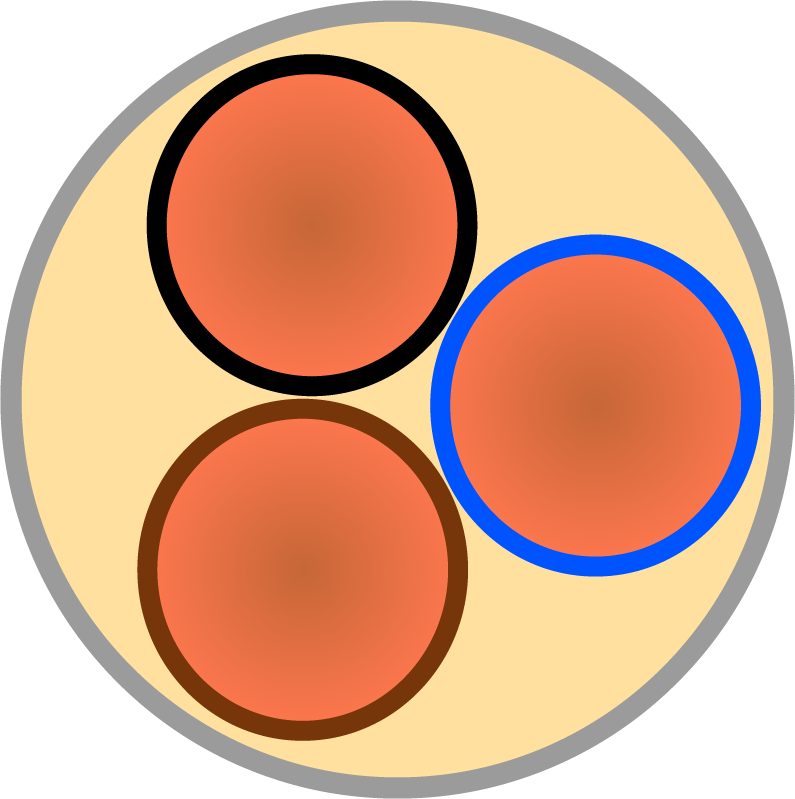
\includegraphics[scale=0.3]{./Bilder/Logo2Klein.png}\\[2ex]

\vspace*{1.65cm}

\normalsize

\copyright \autor \jahr

Besuchen Sie auch die Webseite zum Dokument! Dort finden Sie News rund ums Thema Leitungsberechnung und vieles mehr! \url{http://www.dieleitungsberechnung.de}

Sollten Sie Fehler in dem Dokument finden oder Verbesserungsvorschl�ge haben: \url{mailto:support@dieleitungsberechnung.de}

\end{center}
\end{titlepage}

\pagenumbering{Roman}
\tableofcontents

% Abk�rzungsverzeichnis
\clearpage\markboth{\nomname}{\nomname} 
\listoffigures					% Abbildungsverzeichnis
\listoftables					% Tabellenverzeichnis

\clearpage
\pagenumbering{arabic}
\printnomenclature

% Inhalt 
\part{Schnellauswahl einer Leitung, ohne aufw�ndige Berechnung im Alltag}
\chapter{Schnellauswahl einer Leitung in der Praxis}
\label{cha:Schnellauswahl einer Leitung in der Praxis}

In der Praxis \index{Praxis} ist es oft nicht m�glich langwierige Berechnungen durch zu f�hren. Daher m�chte ich Standard Tabellen zeigen, damit einfacher Leitungsquerschnitte\index{Leitungsquerschnitte} ermittelt werden k�nnen. Allerdings ist es wichtig, dass bei der Ermittlung immer die Randbedingungen beachtet werden!

\section{Wie benutze ich die Tabellen?}
\label{cha:Wie benutze ich die Tabellen?}

Die Benutzung der Tabellen ist vergleichsweise einfach, im Gegensatz zu den aufw�ndigeren Berechnungen. Es gibt hier nur zwei Schritte die zu erledigen sind. Zu beachten ist, dass WS hierbei f�r Wechselstrom und DS f�r Drehstrom steht. Aus Platzgr�nden mussten die Abk�rzungen gew�hlt werden. 

\begin{itemize}
\item \textbf{Schritt 1:} In dem Schritt ermitteln wir den Querschnitt zur eingebauten Sicherung. Dieses machen wir mit den Tabellen in Kapitel \ref{cha:Auswahl nach der Belastbarkeit}. Wir schauen bei der jeweiligen Verlegeart und suchen die Sicherung. An der linken Seite steht nun der zu Verlegende \index{Querschnitt}Querschnitt.
\item \textbf{Schritt 2:} In Kapitel \ref{cha:Auswahl nach dem Spannungsfall} k�nnen Sie mit dem ermittelten Querschnitt und der Sicherung die L�nge der Leitung ermitteln. Nun wissen Sie sofort welchen Querschnitt Sie verlegen m�ssen und welche L�nge die Leitung haben darf.
\end{itemize}

Achtung, da diese Berechnungen sich auf viele Randbedingungen verlassen ist eine Verifikation vor Ort unbedingt notwendig. Besonders wichtig ist hierbei die Berechnung des Kurzschlussschutzes. Die gesamten Tabellen gelten f�r Kabel und Leitungen aus Kupfer.

\section{Auswahl nach der Belastbarkeit}
\label{cha:Auswahl nach der Belastbarkeit}

Die Tabellen \ref{tab:Absicherungen ohne H�ufung} und \ref{tab:Absicherungen mit H�ufung} zeigen die maximal m�gliche \index{Absicherung}Absicherung eines Querschnittes bei der jeweiligen Verlegeart. Hierbei sind folgende Bedingungen zu beachten:

\begin{itemize}
\item Temperatur 30�C
\item Keine H�ufung von anderen Leitungen
\end{itemize}

\begin{table}[htbp]
\caption{Absicherungen ohne H�ufung}
\label{tab:Absicherungen ohne H�ufung}
\centering
\begin{tabular}{||>{\centering}m{3 cm}||>{\centering}m{1,7 cm}||>{\centering}m{1,7 cm}||>{\centering}m{1,7 cm}||>{\centering}m{1,7 cm}||>{\centering}m{1,7 cm}||c||}
\hline 
\centering Verlegeart & \multicolumn{2}{|>{\centering}m{4 cm}||}{Mehraderleitung in Rohr in W�rmeged�mter Wand} & \multicolumn{2}{|>{\centering}m{4 cm}||}{Mehraderleitung in Rohr auf der Wand} & \multicolumn{2}{|>{\centering}m{4 cm}||}{Ein-mehradriges Kabel direkt auf der Wand}\\
\hline \begin{tabular}{c} Versorgungsart \\ \hline Querschnitt\\ \end{tabular} & WS & DS & WS & DS & WS & DS\\ 
\hline\hline 1,5 mm\textsuperscript{2} & 13 A & 13 A & 16 A & 13 A & 16 A & 16 A\\ 
\hline 2,5 mm\textsuperscript{2} & 16 A & 16 A & 20 A & 20 A & 25 A & 20 A\\ 
\hline 4 mm\textsuperscript{2} & 25 A & 20 A & 25 A & 25 A & 32 A & 32 A\\ 
\hline 6 mm\textsuperscript{2} & 32 A & 25 A & 32 A & 32 A & 32 A & 32 A\\ 
\hline 10 mm\textsuperscript{2} & 32 A & 32 A & 50 A & 32 A & 63 A & 50 A\\ 
\hline 16 mm\textsuperscript{2} & 50 A & 50 A & 63 A & 50 A & 80 A & 63 A\\ 
\hline 25 mm\textsuperscript{2} & 80 A & 63 A & 80 A & 80 A & 100 A & 80 A\\ 
\hline 35 mm\textsuperscript{2} & 80 A & 80 A & 100 A & 80 A & 125 A & 100 A\\ 
\hline
\end{tabular} 
\end{table}

\begin{itemize}
\item Temperatur 30�C
\item Mit H�ufung von anderen Leitungen
\end{itemize}

\begin{table}[htbp]
\caption{Absicherungen mit H�ufung}
\label{tab:Absicherungen mit H�ufung}
\centering
\begin{tabular}{||>{\centering}m{3 cm}||>{\centering}m{1,7 cm}||>{\centering}m{1,7 cm}||>{\centering}m{1,7 cm}||>{\centering}m{1,7 cm}||>{\centering}m{1,7 cm}||c||}
\hline 
\centering Verlegeart & \multicolumn{2}{|>{\centering}m{4 cm}||}{Mehraderleitung in Rohr in W�rmeged�mter Wand} & \multicolumn{2}{|>{\centering}m{4 cm}||}{Mehraderleitung in Rohr auf der Wand} & \multicolumn{2}{|>{\centering}m{4 cm}||}{Ein-mehradriges Kabel direkt auf der Wand}\\
\hline \begin{tabular}{c} Versorgungsart \\ \hline Querschnitt\\ \end{tabular} & WS & DS & WS & DS & WS & DS\\ 
\hline\hline 1,5 mm\textsuperscript{2} & 6 A & 6 A & 10 A & 6 A & 10 A & 10 A\\ 
\hline 2,5 mm\textsuperscript{2} & 10 A & 10 A & 13 A & 13 A & 16A & 13 A\\ 
\hline 4 mm\textsuperscript{2} & 16 A & 13 A & 16 A & 16 A & 20 A & 20 A\\ 
\hline 6 mm\textsuperscript{2} & 20 A & 16 A & 20 A & 20 A & 20 A & 20 A\\ 
\hline 10 mm\textsuperscript{2} & 20 A & 20 A & 32 A & 20 A & 32 A & 32 A\\ 
\hline 16 mm\textsuperscript{2} & 32 A & 32 A & 32 A & 32 A & 50 A & 32 A\\ 
\hline 25 mm\textsuperscript{2} & 50 A & 32 A & 50 A & 50 A & 63 A & 50 A\\ 
\hline 35 mm\textsuperscript{2} & 50 A & 50 A & 63 A & 50 A & 80 A & 63 A\\ 
\hline
\end{tabular} 
\end{table}

\section{Auswahl nach dem Spannungsfall}
\label{cha:Auswahl nach dem Spannungsfall}

\subsection{Leitungsl�ngen zu Verbrauchern}
\label{cha:Leitungsl�ngen zu Verbrauchern}

Die erste Tabelle \ref{tab:Leitungsl�ngen bei Wechselstrom} zeigt die maximal erlaubten L�ngen bei einem normalen Wechselstromverbraucher mit einer Spannung von $ U = 230\,\text{V} $. Hierbei sind die Leitungen direkt zur Hauptverteilung verlegt, da hier mit einem \index{Spannungsfall}Spannungsfall von $ \Delta u = 3\,\text{\%} $ gerechnet wurde. Ebenfalls sind ohmsche Verbraucher angeschlossen.

\begin{table}[htbp]
\caption{Leitungsl�ngen bei Wechselstrom}
\label{tab:Leitungsl�ngen bei Wechselstrom}
\centering
\begin{tabular}{||c||c||c||c||c||c||c||c||}
\hline \begin{tabular}{c} Querschnitt \\ \hline Sicherungsgr��e\\ \end{tabular}  & 1,5 mm\textsuperscript{2} & 2,5 mm\textsuperscript{2} & 4 mm\textsuperscript{2} & 6 mm\textsuperscript{2} & 10 mm\textsuperscript{2} & 16 mm\textsuperscript{2} & 25 mm\textsuperscript{2}\\ 
\hline \hline 10 A &  29,0 m & 48,3 m & 77,3 m & 115,9 m & 193,2 m & 309,1 m & 483,0 m \\
\hline 16 A & 18,1 m & 30,2 m & 48,3 m & 72,5 m & 120,8 m & 193,2 m & 301,9 m \\
\hline 20 A & 14,5 m & 24,2 m & 38,6 m & 58,0 m & 96,6 m & 154,6 m & 241,5 m \\
\hline 25 A & 11,6 m & 19,3 m & 30,9 m & 46,4 m & 77,3 m & 123,6 m & 193,2 m \\
\hline 32 A & 9,1 m & 15,1 m & 24,2 m & 36,2 m & 60,4 m & 96,6 m & 150,9 m \\
\hline 35 A & 8,3 m & 13,8 m & 22,1 m & 33,1 m & 55,2 m & 88,3 m & 138,0 m \\
\hline 50 A & 5,8 m & 9,7 m & 15,5 m & 23,2 m & 38,6 m & 61,8 m & 96,6 m \\
\hline 63 A & 4,6 m & 7,7 m & 12,3 m & 18,4 m & 30,7 m & 49,1 m & 76,7 m \\
\hline 
\end{tabular} 
\end{table}

Die zweite Tabelle \ref{tab:Leitungsl�ngen bei Drehstrom} zeigt die maximal erlaubten L�ngen bei einem normalen Drehstromverbraucher mit einer Spannung von $ U = 400\,\text{V} $. Hierbei sind die Leitungen direkt zur Hauptverteilung verlegt, da hier mit einem Spannungsfall von $ \Delta u = 3\,\text{\%} $ gerechnet wurde. Ebenfalls sind ohmsche Verbraucher angeschlossen.

\begin{table}[htbp]
\caption{Leitungsl�ngen bei Drehstrom}
\label{tab:Leitungsl�ngen bei Drehstrom}
\centering
\begin{tabular}{||c||c||c||c||c||c||c||c||}
\hline \begin{tabular}{c} Querschnitt \\ \hline Sicherungsgr��e\\ \end{tabular}  & 1,5 mm\textsuperscript{2} & 2,5 mm\textsuperscript{2} & 4 mm\textsuperscript{2} & 6 mm\textsuperscript{2} & 10 mm\textsuperscript{2} & 16 mm\textsuperscript{2} & 25 mm\textsuperscript{2}\\ 
\hline \hline 10 A &  58,2 m & 97,0 m & 155,2 m & 232,8 m & 388,0 m & 620,8 m & 969,9 m \\
\hline 16 A & 36,4 m & 60,6 m & 97,0 m & 145,5 m & 242,5 m & 388,0 m & 606,2 m \\
\hline 20 A & 29,1 m & 48,5 m & 77,6 m & 116,4 m & 194,0 m & 310,4 m & 485,0 m \\
\hline 25 A & 23,3 m & 38,8 m & 62,1 m & 93,1 m & 155,2 m & 248,3 m & 388,0 m \\
\hline 32 A & 18,2 m & 30,3 m & 48,5 m & 72,7 m & 121,2 m & 194,0 m & 303,1 m \\
\hline 35 A & 16,6 m & 27,7 m & 44,3 m & 66,5 m & 110,9 m & 177,4 m & 277,1 m \\
\hline 50 A & 11,6 m & 19,4 m & 31,0 mm & 46,6 m & 77,6 m & 124,2 m & 194,0 m \\
\hline 63 A & 9,2 m & 15,4 m & 24,6 m & 37,0 m & 61,6 m & 98,5 m & 154,0 m \\
\hline 
\end{tabular} 
\end{table}

\subsection{Leitungsl�ngen zu Unterverteilungen}
\label{cha:Leitungsl�ngen zu Unterverteilungen}

Wichtig sind auch die \index{Leitungsl�ngen zu Unterverteilungen}Leitungsl�ngen zu Unterverteilungen. Hierbei ist zu beachten, dass hier nur ein geringer Teil des gesamten Spannungsfalls abfallen darf.

\begin{table}[htbp]
\caption{Leitungsl�ngen zu Unterverteilungen}
\label{tab:Leitungsl�ngen zu Unterverteilungen}
\centering
\begin{tabular}{||c||c||c||c||c||c||c||c||}
\hline \begin{tabular}{c} Querschnitt \\ \hline Sicherungsgr��e\\ \end{tabular} & 1,5 mm\textsuperscript{2} & 2,5 mm\textsuperscript{2} & 4 mm\textsuperscript{2} & 6 mm\textsuperscript{2} & 10 mm\textsuperscript{2} & 16 mm\textsuperscript{2} & 25 mm\textsuperscript{2} \\
\hline\hline 10 A & 19,4 m & 32,3 m & 51,7 m & 77,6 m & 129,3 m & 206,9 m & 323,3 m \\
\hline 16 A & 12,1 m & 20,2 m & 32,3 m & 48,5 m & 80,8 m & 129,3 m & 202,1 m \\
\hline 20 A & 9,7 m & 16,2 m & 25,9 m & 38,8 m & 64,7 m & 103,5 m & 161,7 m \\
\hline 25 A & 7,8 m & 12,9 m & 20,7 m & 31,0 m & 51,7 m & 82,8 m & 129,3 m \\
\hline 32 A & 6,1 m & 10,1 m & 16,2 m & 24,2 m & 40,4 m & 64,7 m & 101,0 m \\
\hline 35 A & 5,5 m & 9,2 m & 14,8 m & 22,2 m & 37,0 m & 59,1 m & 92,4 m \\
\hline 50 A & 3,9 m & 6,5 m & 10,3 m & 15,5 m & 25,9 m & 41,4 m & 64,7 m \\
\hline 63 A & 3,1 m & 5,1 m & 8,2 m & 12,3 m & 20,5 m & 32,8 m & 51,3 m \\
\hline

\end{tabular} 
\end{table}
\part{Ausf�hrliche Dimensionierung eine Leitung}
\chapter{Grundlagen}
\label{cha:Kapitel1}

F�r die Berechnung einer Leitung sind einige wichtige Kenntnisse erforderlich. In diesem Dokument werden die wichtigsten Kenntnisse vermittelt, um alle weiteren Kapitel zu verstehen. Hierzu wird ausf�hrlich die Funktionweise von Sicherungen beschrieben.

Ein jeder Verbraucher dessen Strom keinen sinusf�rmigen Verlauf mehr hat, wird von Netzoberwellen �berlagert. Die Oberwellen k�nnen auch in Privathaushalten zu einer Neutralleiter�berlastung f�hren. Insbesondere in der Industrie k�nnen Oberwellen, unter anderem durch Schaltnetzteile in Computern, Servern, EVGs in Leuchtstofflampen verursacht, zu einer �berlastung des \index{Neutralleiter}Neutralleiters f�hren. In diesem Dokument wird den Oberwellen keine Beachtung geschenkt.

Dieses Dokument, das Dokument zu dem \index{Oberwellen}Oberwellen, ein Programm um eine Leitung zu berechnen und vieles mehr finden Sie auf der Webseite zum Dokument:
\url{http://www.dieleitungsberechnung.de}

\section{Rechtliche Grundlagen / Haftungsausschluss}
\label{cha:Rechtliche Grundlagen / Haftungsausschluss}

Es wird keine Haftung �bernommen, f�r fehlerhafte Leitungsberechnung sowie fehlerhafte Leitungsverlegung. Au�erdem wird keine Haftung f�r die technische Korrektheit des Dokuments �bernommen, da dieses Dokument lediglich als Beispiel zu verstehen ist. Des Weiteren d�rfen Kabel und Leitungen nur von Fachleuten verlegt werden. Das Verlegen von Kabeln und Leitungen durch Laien ist eindeutig verboten! Siehe dazu das folgende Zitat aus der NAV\footnote{NAV \S13 Absatz 2}:
\begin{quote}
(2) Unzul�ssige R�ckwirkungen der Anlage sind auszuschlie�en. Um dies zu gew�hrleisten, darf die Anlage nur nach den Vorschriften dieser Verordnung, nach anderen anzuwendenden Rechtsvorschriften und beh�rdlichen Bestimmungen sowie nach den allgemein anerkannten Regeln der Technik errichtet, erweitert, ge�ndert und instand gehalten werden. In Bezug auf die allgemein anerkannten Regeln der Technik gilt � 49 Abs. 2 Nr. 1 des Energiewirtschaftsgesetzes entsprechend. Die Arbeiten d�rfen au�er durch den Netzbetreiber nur durch ein in ein Installateurverzeichnis eines Netzbetreibers eingetragenes Installationsunternehmen durchgef�hrt werden; im Interesse des Anschlussnehmers darf der Netzbetreiber eine Eintragung in das Installateurverzeichnis nur von dem Nachweis einer ausreichenden fachlichen Qualifikation f�r die Durchf�hrung der jeweiligen Arbeiten abh�ngig machen. Mit Ausnahme des Abschnitts zwischen Hausanschlusssicherung und Messeinrichtung einschlie�lich der Messeinrichtung gilt Satz 4 nicht f�r Instandhaltungsarbeiten.
\end{quote}

In diesem Abschnitt ist eindeutig geregelt, dass eine Installation nur durch eine Fachkraft ausgef�hrt werden darf. Daher wird jegliche Haftung ausgeschlossen, sollten die Leitungen nicht fachgerecht, sondern laienhaft verlegt werden.

\section{Grundlagen Leitungsschutzschalter (LSS)}
\label{cha:Grundlagen Leitungsschutzschalter}

\begin{figure}[htbp]
\centering
\includegraphics[width=0.3\textwidth]{../Bilder/UnterlagenHager/MBN116}
\caption{Leitungsschutzschalter Typ B16 A (von \cite{hager2012})}
\label{fig:MBN116}
\end{figure}

Das Bild \ref{fig:MBN116} zeigt einen \index{Leitungsschutzschalter}Leitungsschutzschalter mit der \index{Charakteristik}Charakteristik B (siehe Kapitel \ref{cha:Funktionsweise Leitungsschutzschalter}) und 16A. Zu sehen ist, dass dieser Leitungsschutzschalter\index{Leitungsschutzschalter} (im weiteren LSS\index{LSS} genannt) einem Schalter �hnelt und keiner Schmelzsicherung\index{Schmelzsicherung}. Die Erl�uterung des genauen technischen Aufbaus findet in den folgenden Kapiteln statt.
\clearpage
Bei Leitungsschutzschaltern sind grunds�tzlich folgende Einschr�nkungen zu beachten:

\begin{itemize}
\item LSS d�rfen nicht benutzt werden, um Motoren zu sch�tzen, dieser Anwendungsfall tritt in privaten Haushalten eher selten auf.
\item LSS sind geeignet, um zum Trennen von Stromkreisen verwendet zu werden. Betriebsm��iges Schalten darf �ber LSS \underline{nicht} erfolgen!
\item \index{Temperaturbereich}Temperaturbereich \unit[-5]{�C} bis \unit[+40]{�C} wobei ein Durchschnittswert von \unit[+35]{�C} innerhalb von 24 h nicht �berschritten werden darf.
\item Der Einbauort muss unter 2000 m NN liegen.
\end{itemize}

Besonders wichtig sind die folgenden Eingenschaften auf die wir in Kapitel \ref{cha:Funktionsweise Leitungsschutzschalter} n�her eingehen.

\begin{itemize}
\item[\textbf{Charakteristik:}]Eingegangen wird auf die Charakteristik B,C sowie D.
\item[\textbf{Nennstrom $ I_{N} $:}]Beschreibt den Strom, welchen die Sicherung dauerhaft halten kann.
\item[\textbf{Kurzschlussschaltverm�gen:}]Ist die H�he des \index{Kurzschlussstrom}Kurzschlussstromes, welcher noch abschaltbar ist.\index{Kurzschlussschaltverm�gen}
\end{itemize}

\subsection{Funktionsweise}
\label{cha:Funktionsweise Leitungsschutzschalter}

Bevor wir die Funktionsweise n�her erl�utern, stellen wir zuerst eine �berlegung an, f�r welche Aufgaben dieser Leitungsschutzschalter gedacht ist. Der Name zeigt deutlich den eigentlichen Zweck auf. Dieses Element ist dazu gedacht die Leitung zu sch�tzen. Wie soll er dies erledigen?

\begin{enumerate}
\item \textbf{�berstrom:} Bei einem zu hohen Stromfluss, verursacht durch zu viele Verbraucher an den Steckdosen, muss der LSS ausschalten. Stellen Sie sich folgende Situation vor: Bei Ihnen arbeitet Ihr Partner \slash  Ihre Partnerin in der K�che und bereitet das Essen zu. Nun m�chten Sie einen Tee trinken. Sobald Sie den Wasserkocher einschalten, l�st die Sicherung aus. Der Strom ist hier auf genau 16,2 A angestiegen, also nur 0,2 A �ber dem erlaubten Wert. Eigentlich arbeitet der LSS korrekt, aber es w�re kein akzeptabler Zustand. Der LSS muss in der Anfangsphase verz�gert ausl�sen, da es einfach inakzeptabel ist, wegen einer kleinen �berlastung die Verteilung aufzusuchen, um die Sicherung wieder einzuschalten.

\item \textbf{Kurzschluss:} Wenn ein Kurzschluss auftritt, so muss der Kurzschluss umgehend abgeschaltet werden. Dies ist die Aufgabe des Leitungsschutzschalters.

\end{enumerate}

Aufgrund dieser �berlegungen k�nnen wir schlussfolgern, dass ein LSS mehrere M�glichkeiten besitzen muss, um die fehlerhaften Zust�nde zu verhindern. Dies ist zum Einem der thermische Ausl�ser, mittels eines Bi-Metalls, und ein magnetischer Ausl�ser.

\begin{figure}[htbp]
\centering
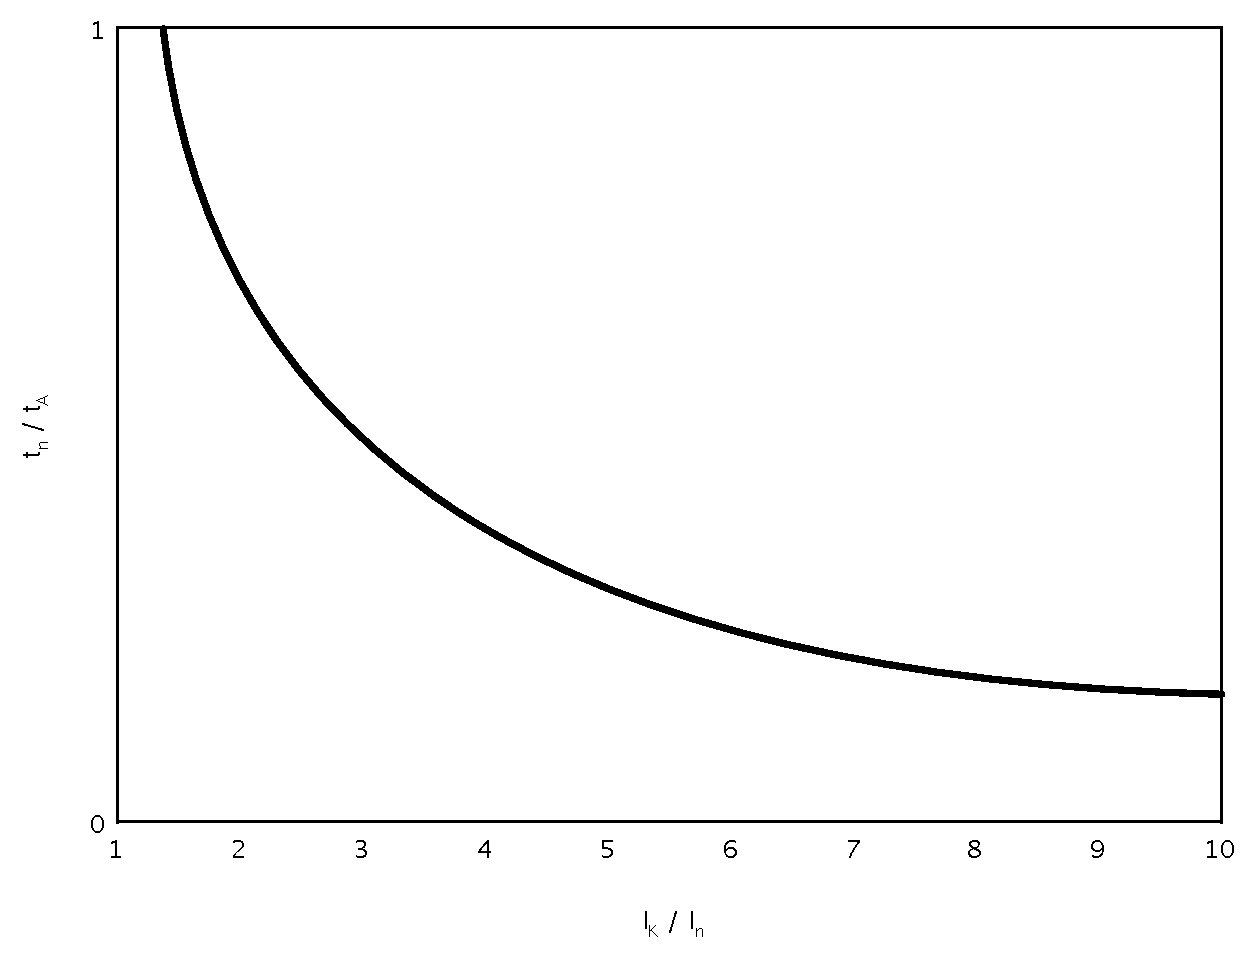
\includegraphics[width=0.8 \textwidth]{../Bilder/Thermischer_Ausloeser.pdf}
\caption{Thermischer Ausl�ser}
\label{fig:Thermischer_Ausloeser}
\end{figure}

Bild \ref{fig:Thermischer_Ausloeser} zeigt eine Kennlinie f�r den thermischen Ausl�ser. Dieser funktioniert mit einem Bi-Metall. Dieses hat die Eigenschaft, dass es sich bei Erw�rmung verbiegt. Eine Eingenschaft, die dieses Metall erh�lt, aufgrund der Verbindung von zwei verschiedenen Metallen. Diese Metalle dehnen sich bei Erw�rmung unterschiedlich aus. Dadurch verbiegt sich das Bi-Metall. Das hat den Vorteil, dass bei langsam ansteigendem Strom der LSS nicht sofort ausl�st. Erw�rmt sich jetzt das Bi-Metall durch einen Strom, so verbiegt es sich und l�st damit die Sicherung aus. Der Stromkreis ist ge�ffnet und der �berstrom abgeschaltet. Dieses Verhalten ist Bild \ref{fig:Thermischer_Ausloeser} zu erkennen. Bei langsam ansteigendem Strom sinkt langsam die Ausl�sezeit. Genau dieses Verhalten ist von uns gew�nscht, damit ein LSS nicht sofort ausl�st.

\begin{figure}[htbp]
\centering
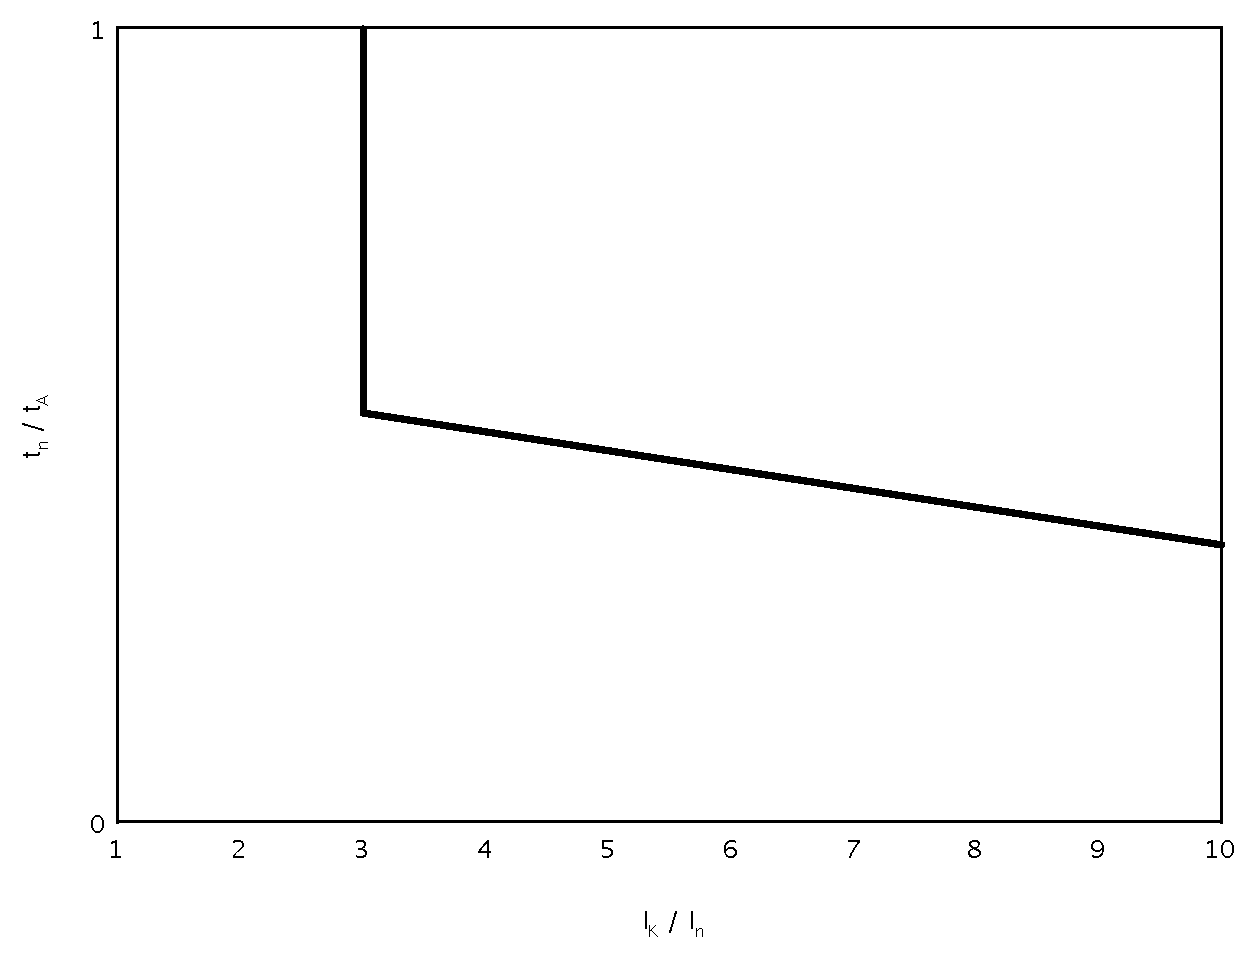
\includegraphics[width=0.8 \textwidth]{../Bilder/Magnetischer_Ausloeser.pdf}
\caption{magnetischer Ausl�ser}
\label{fig:Magnetischer_Ausloeser}
\end{figure}

Betrachten wir das Bild \ref{fig:Magnetischer_Ausloeser}. Dort ist ersichtlich, dass bis zum dreifachen Nennstrom nichts passiert und dann der LSS ausl�st. Hier ist die Schaltschwelle �berschritten wurden. Der magnetische Ausl�ser spricht an und bringt den LSS schnellstm�glich zum Ausl�sen. Das Ausl�sen geschieht �ber ein magnetisches Feld. Der magnetische Ausl�ser besitzt einen Kennwert bei dem er ausl�st. Hierbei wird das Magnetfeld ausreichend stark, damit ein Kontakt �ffnen kann. Zus�tzlich ist eine sogenannte Funkbogenl�schkammer\index{Funkbogenl�schkammer} in der Sicherung eingebaut. Sollte die Sicherung ausschalten, so kann ein Lichtbogen entstehen. Damit die Sicherung nicht besch�digt wird, muss dieser Lichtbogen gel�scht werden.

Wenn nun beide Bilder \ref{fig:Magnetischer_Ausloeser} und \ref{fig:Thermischer_Ausloeser} zusammengef�gt werden, dann erhalten wir im Ergebnis die Kennlinien im Bild \ref{fig:Zeit-Strom-Diagramm f�r Leitungsschutzschalter}. Dieses Bild zeigt drei LSS der Kategorien B,C und D. Diese besitzen alle unterschiedliche Kennwerte. Die genauen Eigenschaften der Zeit-Strom-Kennlinie werden in Kapitel \ref{cha:Zeit-Strom-Diagramm Leitungsschutzschalter} beschrieben.

Eine wichtige Gr��e ist das Bemessungsschaltverm�gen\index{Bemessungsschaltverm�gen}. In Bild \ref{fig:MBN116} ist es durch ein Rechteck mit einer gro�en Zahl gekennzeichnet. Es befindet sich die Zahl 6000 in einem Rechteck. Diese gibt an, wie hoch der maximale Kurschlussstrom sein darf, welcher zum flie�en kommt (hier 6000 A). Sollte dieser Strom �berschritten werden, so kann eine korrekte Funktionsweise nicht mehr garantiert werden. Es muss also zwingend darauf geachtet werden, dass die eingesetzten Ger�te eine h�heres Bemessungsschaltverm�gen besitzen als die H�he des auftretenden Kurzschlussstromes angibt. F�r Leitungsschutzschalter welche direkt einem Endstromkreis sch�tzen, muss mindestens ein Bemessungsschaltverm�gen von 6000 A verbaut sein.

\subsection{Zeit-Strom-Diagramm}
\label{cha:Zeit-Strom-Diagramm Leitungsschutzschalter}

Das Bild \ref{fig:Zeit-Strom-Diagramm f�r Leitungsschutzschalter} zeigt das \index{Zeit-Strom-Diagramm}Zeit-Strom-Diagramm der Leitungsschutzschalter. Sehr gut sind die einzelnen Charakteristiken zu erkennen, welche bereits in Kapitel \ref{cha:Funktionsweise Leitungsschutzschalter} angesprochen wurden. 

\begin{figure}[htbp]
\centering
\includegraphics[width=0.8 \textwidth]{../Bilder/UnterlagenHager/Ausloese_001i_MGS_D}
\caption{Zeit-Strom-Diagramm f�r Leitungsschutzschalter (von \cite{hager2012})}
\label{fig:Zeit-Strom-Diagramm f�r Leitungsschutzschalter}
\end{figure}

Auch die beiden F�lle, thermischer sowie \index{magnetischer Ausl�ser}magnetischer Ausl�ser sind in den Kennlinien zu sehen. Bei Betrachtung der Charakteristik B ist ersichtlich, dass diese beim dreifachen Nennstrom den Stromkreis trennt. Die Kennlinie geht hier bis zum f�nf fachen des Nennstroms. Dieser Bereich ist gekennzeichnet durch das Abschalten mittels magnetischen Ausl�ser. Der vorherige Bereich wird mittels des \index{thermischer Ausl�ser}thermischen Ausl�sers abgeschaltet. Bei den Charakteristiken C und D ist es �hnlich. Lediglich die Werte des magnetischen Ausl�sers unterscheiden sich. Dies wiederum ist das wichtigste Unterscheidungskriterium der einzelnen Charakteristiken. Die beiden Einfassungen des magnetischen Ausl�sers zeigen das sichere Abschalten des LSS bei bestimmten Zeiten. Die Tabelle \ref{tab:Abschaltzeiten der Leitungsschutzschalter-Charakteristiken} zeigt eine �bersicht �ber diese Zeiten und Str�me.

\begin{table}[htbp]
\caption{Abschaltzeiten der Leitungsschutzschalter-Charakteristiken}
\label{tab:Abschaltzeiten der Leitungsschutzschalter-Charakteristiken}
\centering
\begin{tabular}{||c||c||c||c||c||c||c||}
\hline Charakteristik &  \multicolumn{2}{|c||}{B}  &  \multicolumn{2}{|c||}{C}  &  \multicolumn{2}{|c||}{D}  \\ \hline
\hline $ t_{A} $ & 5 s & 0,1 s & 5 s & 0,1 s & 5 s & 0,1 s \\ 
\hline $ I_{N} / I_{K} $ & 3 & 5 & 5 & 10 & 10 & 20 \\ 
\hline 
\end{tabular} 
\end{table}

Die \index{Pr�fstr�me}Pr�fstr�me geben an, wie lange ein definierter Strom flie�en kann, um den Leitungsschutzschalter in einer definierten Zeit zum Ausl�sen zu bringen. Diese Str�me sind zum Testen des magnetischen Ausl�sers wichtig. Die Tabelle \ref{tab:Pr�fstr�me der Leitungsschutzschalter} zeigt die Pr�fstr�me der drei Charakteristiken B, C sowie D.

Kleiner Pr�fstrom $ I_{1} $ muss in der Zeit $ t > 1h $ ausl�sen.

\begin{equation}
I_{1} = 1,13 \cdot I_{N}
\end{equation}


Gro�er Pr�fstrom $ I_{2} $ muss in der Zeit $ t < 1h $ ausl�sen.

\begin{equation}
I_{2} = 1,45 \cdot I_{N}
\end{equation}

 
 \begin{table}[htbp]
 \caption{Pr�fstr�me der Leitungsschutzschalter}
 \label{tab:Pr�fstr�me der Leitungsschutzschalter}
 \centering
 \begin{tabular}{||c||c||c||c||}
  \hline Was & LSS Typ B & LSS Typ C & LSS Typ D \\ 
  \hline \hline Kleiner Pr�fstrom $ I_{1} $ & 1,13 & 1,13 & 1,13  \\ 
  \hline Gro�er Pr�fstrom $ I_{2} $ & 1,45 & 1,45 & 1,45 \\
  \hline
  \end{tabular} 
 \end{table}

\subsection{Verwendung des Zeit-Strom-Diagramms}
\label{cha:Verwendung des Zeit-Strom-Diagramms Leitungsschutzschalter}

Die Verwendung der Kennlinien ist ziemlich einfach. Es gibt zwei Dinge die man unterscheiden muss. Die verschiedenen Arten des Ausl�sens (magnetisch sowie thermisch)  m�ssen bei dem Ablesen der Werte ber�cksichtigt werden.

Das ablesen des thermischen Ausl�sers soll Anhand eines Beispiels veranschaulicht werden. Folgende Daten sind uns bekannt:

\begin{list}{}{}
\item $ I_{N} = 10\,\text{A} $
\item $ I_{K} = 15\,\text{A} $
\end{list}

Wir suchen die Zeit, welche die Sicherung ben�tigt um den Strom weg zu schalten. Wie k�nnen ein Vielfaches des Nennstromes mit $ \frac{I_{K}}{I_{N}} = 1,5$ berechnen. Damit loten wir auf der Kennlinie nach oben, bis wir auf die Kennlinie der Sicherung sto�en. Dort lesen wir die Zeit von $ t_{A} = 400\,\text{s} $ ab.

\begin{figure}[!h]
\centering
\includegraphics[width=0.449\textwidth]{../Bilder/UnterlagenHager/LSS_Auslesen}
\caption{Ablesen des Zeit-Strom-Diagramm eines LSS (Diagramm von \cite{hager2012})}
\label{fig:LSS_Auslesen}
\end{figure}

Der magnetische Ausl�ser ist noch einfacher. Hierzu ist lediglich ein Blick in Tabelle \ref{tab:Abschaltzeiten der Leitungsschutzschalter-Charakteristiken} n�tig. �bersteigt das vielfache des Nennstromes die Werte in der Tabelle \ref{tab:Abschaltzeiten der Leitungsschutzschalter-Charakteristiken}, so sind die entsprechenden Abschaltzeiten in der Spalte zu nutzen.

\section{Grundlagen Schmelzsicherungen}
\label{cha:Grundlagen Schmelzsicherungen}

\subsection{Funktionsweise}
\label{cha:Funktionsweise Schmelzsicherung}
\index{Schmelzsicherung}
Die Funktionsweise ist verh�ltnism��ig einfach. In einem Porzellank�rper befindet sich ein Draht und Quarzsand. Nachfolgend die Erkl�rung der einzelnen Komponenten:

\begin{itemize}
\item \textbf{Porzellank�rper:} Dient als stabiler Rahmen der Sicherung. Gleichzeitig ist es in der Lage, die hohe Temperaturen bei einem Kurschluss zu verkraften.
\item \textbf{Draht:} Dieser Draht ist das Herzst�ck der Sicherung. Dieser ist so dimensioniert, dass dieser Draht bei einem definierten Strom in einer definierten Zeit schmilzt. Wann diese Zeiten und Str�me sind zeigt Bild \ref{fig:Zeit-Strom-Diagramm Schmelzsicherung}. \index{Zeit-Strom-Diagramm Schmelzsicherung}�bersteigt ein Strom nun den erlaubten Grenzen des Drahtes, so wird der Draht so hei� das dieser schmilz und den Stromkreis unterbricht. Das ist das Geheimnis der Schmelzsicherung.
\item \textbf{Quarzsand:} Bei dem Schmelzen des Drahtes kann es zu einem \index{Lichtbogen}Lichtbogen kommen. Dieser wird durch den Quarzsand gel�scht und somit der Stromkreis ge�ffnet.
\end{itemize}



\subsection{Zeit-Strom-Diagramm}
\label{cha:Zeit-Strom-Diagramm Schmelzsicherung}

Das in Bild \ref{fig:Zeit-Strom-Diagramm Schmelzsicherung} abgebildete Zeit-Strom-Diagramm zeigt gL-gG Schmelzsicherungen. Die Wichtigsten sind in dieser Kennlinie abgebildet. Auch diese Sicherung hat einen \index{Pr�fstrom}Pr�fstrom, welchen die Sicherung eine definierte Zeit lang halten muss. Wichtig ist weiterhin auch die logarithmische Achsteilung zu achten.

Gro�er Pr�fstrom $ I_{2} $ muss in der Zeit $ t < 1\,\text{h} $ ausl�sen.
\begin{equation}
 I_{2} = 1,45 \cdot I_{N} 
\end{equation}

\begin{figure}[htbp]
\centering
\includegraphics[width=0.95 \textwidth]{../Bilder/UnterlagenHager/Zeit_Stromkenn_001i}
\caption{Zeit-Strom-Diagramm Schmelzsicherung (von \cite{hager2012})}
\label{fig:Zeit-Strom-Diagramm Schmelzsicherung}
\end{figure}

\subsection{Verwendung des Zeit-Strom-Diagramms}
\label{cha:Verwendung des Zeit-Strom-Diagramms Schmelzsicherung}

Es werden beliebige Werte gew�hlt, um die Umgangsweise zu verdeutlichen.

Der Kurzschlussstrom betr�gt $ I_{K} = 200\,\text{A} $

Die Abschaltzeit $ t_{A} = 20\,\text{ms} $

Es wird die Sicherung gesucht, die bei diesen Werten nicht ausl�st und somit in den Stromkreis eingebracht werden kann. In Abbildung \ref{fig:ZSK_gLgG_Ablesen} werden nun zwei Markierungen eingebracht f�r den jeweiligen Strom und die jeweilige Zeit.

\begin{figure}[htbp]
\centering
\includegraphics[width=1\textwidth]{../Bilder/UnterlagenHager/ZSK_gLgG_Ablesen}
\caption{Ablesen des Zeit-Strom-Diagramm einer Schmelzsicherung (Diagramm von \cite{hager2012})}
\label{fig:ZSK_gLgG_Ablesen}
\end{figure}

Wie man in dem Bild \ref {fig:ZSK_gLgG_Ablesen} sieht, liegt der Schnittpunkt genau auf der Kennlinie der 16 A Sicherung. Sollte dies nicht der Fall sein, so ist die n�chst kleine Sicherung zu w�hlen. Also jene Kennlinie, welche n�her an der Zeitachse liegt.

\clearpage

\section{Grundlagen der Energieversorgungsnetze}
\label{cha:Grundlagen der Energieversorgungsnetze}

\subsection{Abschaltzeiten im �ffentlichen Versorgungsnetz}
\label{cha:Abschaltzeiten im �ffentlichen Versorgungsnetz}

\begin{table}[htbp]
\caption{Abschaltzeiten}
\label{tab:Abschaltzeiten}
\centering
\begin{tabular}{||c||c||c||c||}
\hline \multicolumn{2}{|c|}{Was} & TN - Netz & TT - Netz \\ 
\hline\hline F�r Endstromkreise bis 32 A & 230 V AC & 0,4 s & 0,2 s \\ 
\hline F�r Endstromkreise bis 32 A & 400 V AC & 0,2 s & 0,07 s \\ 
\hline \multicolumn{2}{|c|}{Verteilungsstromkreis und Stromkreis > 32 A} & 5 s & 1 s \\ 
\hline \multicolumn{2}{|c|}{Motorstromkreis} & 5 s & 5 s \\ 
\hline 
\end{tabular}
\end{table}

In der neuen VDE 0100 Teil 410 wurden auch die \index{Abschaltzeiten}Abschaltzeiten f�r die \index{Versorgungsnetze}Versorgungsnetze neu geregelt. Es ist f�r die Ermittlung des Kurzschlussschutzes wichtig, dass die Abschaltzeiten bekannt sind. Es wird in Kapitel \ref{cha:Kapitel4} auf diese Werte eingegangen.

Endstromkreise sind Stromkreise mit fest angeschlossenen Betriebsmitteln oder Betriebsmitteln die �ber eine Steckvorrichtung versorgt werden. Verteilungsstromkreise haben keine direkt angeschlossenen Betriebsmittel, sondern dienen lediglich zur Verteilung der elektrischen Energie. In Motorstromkreisen muss zwischen zwei Situationen unterschieden werden:

\begin{enumerate}
\item Die Installation des Motors in der Industrie. Es kann hierbei davon ausgegangen werden, dass bei einer definierten Steckvorrichtung oder bei einem Festanschluss genau ein Ger�t betrieben wird. Somit gelten hier immer die Abschaltzeiten aus Tabelle \ref{tab:Abschaltzeiten} - Motorstromkreise (auch hier ist Vorsicht geboten und erfordert meistens eine genaue Besichtigung vor Ort!).
\item Geht man im Privathaushalt von fest angeschlossenen Motoren aus, haben sie die oben genannten Abschaltzeiten. Werden die Motoren jedoch �ber Steckvorrichtungen angeschlossen, so gelten hier nicht mehr die Abschaltzeiten f�r Motoren, sondern die Abschaltzeiten der normalen Stromkreise. Dies hat einen einfachen Hintergrund. Es kann in einem Privathaushalt nicht davon ausgegangen werden, dass die Steckvorrichtung lediglich f�r den Motor genutzt wird. Die Zuleitung f�r die Steckvorrichtung muss so angepasst werden, dass sie in jeden Betriebsfall rechtzeitig bei einem Kurzschluss oder im �berstromfall abschaltet.
\end{enumerate}

\section{Idealisierte Berechnungen}
\label{cha:Idealisierte Berechnungen}

In den folgenden Berechnungen wird von den folgenden \index{idealisierten Bedingungen}idealisierten Bedingungen ausgegangen: $ \cos\varphi = 1 $.

Bei dieser idealisierten Betrachtung werden keine imagin�ren Widerst�nde der Kabel und Leitungen ber�cksichtigt. F�r die weiteren Berechnungen werden nur die ohmschen Anteile der Leitungen betrachtet. Dadurch ergibt sich eine Vereinfachung der Rechnung. 

F�r weitere Berechnungen gelten also:
\begin{equation}
\cos\varphi = 1 \Rightarrow R = Z
\end{equation}
Diese idealisierte Berechnung wird nicht f�r die Ermittlung des Betriebsstroms des Ger�tes angewendet. Es erg�be sich dort ein zu gro�er Rechenfehler, der in den weiteren Berechnungen gravierende Auswirkungen h�tte.

Des Weiteren werden einige Berechnungen unter idealisierten Betriebsbedingungen betrachtet und unter vereinfachten Bedingungen Sicherungen ausgew�hlt. Dieses Dokument soll lediglich als grobe Linie f�r die Berechnung dienen und daher wird an vielen Stellen mit idealen Bedingungen gerechnet. Dieses Dokument kann nicht die genaue Besichtigung vor Ort ersetzten!

\chapter{Auswahl der Sicherung}
\label{cha:Kapitel2}

F�r die Auswahl der Sicherung ist es wichtig, die technischen Daten des Ger�tes zu kennen, um somit die Betriebsstromaufnahme des Ger�tes zu ermitteln. Im Folgenden wird hier auf zwei wichtige Auswahlmethoden eingegangen:

\begin{enumerate}
\item Auswahl der Sicherung bei normalen Verbrauchern beispielsweise der Waschmaschine
\item Auswahl der Sicherung in Motorstromkreisen
\end{enumerate}

\section{Ermittlung des Betriebsstroms des Ger�tes}

\begin{equation}
I_{B} = \frac{P_{AB}}{\eta\cdot\cos\varphi\cdot U \cdot X}
\label{eq:Betriebsstrom}
\end{equation}

\begin{list}{}{Bedeutung der einzelnen Elemente:}
\item $ I_{B} $ = Betriebsstrom des Ger�tes
\item $ \cos\varphi $ = Leistungsfaktor des Ger�tes
\item $ X = \sqrt{3} $ bei einem Drehstromverbraucher und 1 bei einem Wechselstromverbraucher
\item $ \eta $ = Wirkungsgrade des Ger�tes
\item $ P_{AB} $ = Abgegebene Leistung des Ger�tes. Wird die aufgenommene Leistung verwendet, ist $ \eta = 1$.
\end{list}

Mit der Formel \ref{eq:Betriebsstrom} kann der Betriebsstrom eines Wechselstromes oder Drehstromverbrauchers ermittelt werden.

\subsection{Beispiel f�r die Ermittlung des Betriebsstroms}

In den folgenden Beispielen werden die beiden oben erw�hnten F�lle behandelt.

\subsubsection{Beispiel f�r einen Drehstromasynchronmotor}

\begin{list}{}{Es wird f�r die Ermittlung ein Drehstromasynchronmotor mit folgenden technischen Daten gew�hlt:}
\item $ \cos\varphi = 0,82 $
\item $ U = 400\,\text{V} $ 
\item $ \eta = 0,9 $
\item $ P_{AB} = 4,8\,\text{kW} $
\end{list}

\[ I_{B} = \frac{P_{AB}}{\eta\cdot\cos\varphi\cdot U \cdot X} = \frac{4,8\,\text{kW}}{0,9 \cdot 0,82 \cdot 400\,\text{V} \cdot\sqrt{3}} = 9,4\,\text{A} \]

Dieser Motor hat also eine Stromaufnahme von $ 9,4\,\text{A} $. Dieser Wert kann jetzt verarbeitet werden.

\subsubsection{Beispiel f�r einen normalen Verbraucher}

\begin{list}{}{F�r die Ermittlung der Stromaufnahme werden die technischen Daten des Ger�tes ermittelt:}
\item $ \cos\varphi = 0,95 $
\item $ U = 230\,\text{V} $ 
\item $ P_{AUF} = 2,5\,\text{kW} $
\end{list}

Da hier die aufgenommene Leistung des Ger�tes angegeben ist, kann der Wirkungsgrad in der Berechnung entfallen.

\[ I_{B} = \frac{P_{AUF}}{\cos\varphi\cdot U \cdot X} = \frac{2,5\,\text{kW}}{0,95 \cdot 230\,\text{V}} = 11,44\,\text{A} \]

Dieses Ger�t hat also eine Stromaufnahme von $ 11,44\,\text{A} $. Dieser Wert kann jetzt verarbeitet werden.

\section{Auswahl der Sicherung}

Die Sicherung wird unter idealen Bedingungen gew�hlt. F�r die Auswahl der Sicherung ist es wichtig, die Stromaufnahme des jeweiligen Ger�tes zu kennen.
\newline
\linebreak
Hierbei ist folgende Bedingung einzuhalten:
\begin{equation}
I_{B}\leq I_{N.Sicherung}
\label{eq:Auswahl Sicherung}
\end{equation}

Der Betriebsstrom des Ger�tes muss niedriger sein als der Nennstrom der Sicherung. Bei den Beispielen wird davon ausgegangen, dass diese Bedingung immer erf�llt ist. Weiterhin ist die Kenntnis des Einschaltstromes, des ohmschen Verbrauchers oder des Motors wichtig. Jedes Ger�t hat in seinem Einschaltmoment einen h�heren Strom als im Betrieb des Ger�tes. Der Einschaltstrom muss nun von der gew�hlten Sicherung gehalten werden, bis dieser Strom wieder abgeklungen ist. Da die Ger�te verschiedene Einschaltstr�me haben k�nnen, kann hier keine generelle Aussage getroffen werden. Die jeweiligen Einschaltstr�me der Ger�te m�ssen f�r eine weitere erfolgreiche Ermittlung der Sicherung bekannt sein, so wie die Zeit, in der der Einschaltstrom zum Flie�en kommt. Es wird folgende Vorgehensweise empfohlen:

\begin{enumerate}
\item Ermittlung des Einschaltstromes
\item Ermittlung der Zeit, in der der Einschaltstrom flie�t
\item Vergleich der Werte mit denen der Sicherungen und Auswahl der passenden Sicherung
\end{enumerate}

Wird in einem Endstromkreis eine Steckvorrichtung angebracht, die der Versorgung verschiedenster Ger�te dienen kann, sollte die Sicherung passend auf den Nennstrom der Steckvorrichtung ausgelegt werden.
\newline
\linebreak
In einem Privathaushalt sollte die Sicherung immer auf den Nennstrom der Steckvorrichtung ausgelegt werden, da hier verschiedenste Ger�te betrieben werden k�nnen. Der Errichter kann hier \textbf{nicht} von dem Betrieb mit einem festen Ger�t ausgehen.
\newline
\linebreak
In der Industrie sieht es anders aus. Hier kann auch bei Steckvorrichtungen von dem Betrieb mit bestimmten Ger�ten ausgegangen werden. Hierbei kann aber keine generelle Aussage getroffen werden, es erfordert eine pers�nliche Begutachtung und Einsch�tzung der Sachlage vor Ort. 

\subsection{Beispiel f�r ein Stromkreis mit ohmschen Verbrauchern, Gl�hlampen}

Es werden an einen Stromkreis Gl�hlampen mit einer Gesamtleitung von $ P = 1035\,\text{W} $ und einem Betriebsstrom von $ I_{B} = 4,5\,\text{A} $ angeschlossen. Die Gl�hlampen haben als Faustregel ca. den 6-fachen Einschaltstrom.

\begin{list}{}
\item $ I_{B} = 4,5\,\text{A} $
\item $ I_{EIN} = 4,5\,\text{A} \cdot 6 = 27\,\text{A} $
\end{list}

Der Einschaltstrom liegt hier bei $ t < 1\,\text{s} $. Die Abschaltzeit des Leitungsschutzschalters bei nicht Erreichen des Kurzschlussstromes ist auf jeden Fall $ t > 1\,\text{s} $. Nun werden diese Daten mit den entsprechenden technischen Daten der Leitungsschutzschalter verglichen.

\begin{table}[h]
\caption{Ansprechen der Leitungsschutzschalter}
\label{tab:Ansprechen der Leitungsschutzschalter}
\centering
\begin{tabular}{||c||c||}
\hline Sicherung & Ansprechen des Kurzschlussschutzausl�sers \\ 
\hline\hline LSS TYP B 6 A & 18 A \\ 
\hline LSS TYP B 10 A &  30 A \\ 
\hline LSS TYP B 16 A & 48 A \\ 
\hline 
\end{tabular}
\end{table}

In Tabelle \ref{tab:Ansprechen der Leitungsschutzschalter} sind die drei m�glichen Kandidaten als Sicherung f�r diesen Stromkreis aufgef�hrt. Die Leitungsschutzschalter der Kategorie B wurden gew�hlt, da in Einfamilienh�usern als Standardabsicherung Leitungsschutzschalter der Kategorie B verwendet werden. Ein Vergleich des Einschaltstromes der Gl�hlampen und dem Ansprechen des Kurzschlussschutzausl�sers zeigt, dass es nicht m�glich ist, eine B 6 A Sicherung zu verwenden. Diese kann den Betriebsstrom zwar halten, jedoch nicht den Einschaltstrom der Verbraucher. Der Leitungsschutzschalter des Typ B 10 A liegt nur minimal �ber dem Einschaltstrom der Gl�hlampen. Er wird in den meisten Einschaltmomenten den Strom halten k�nnen, jedoch gibt es auch hier Schwankungen in der Qualit�t und somit im Ansprechen des Kurzschlussschutzausl�sers. Bei den Gl�hlampen kann es durch Qualit�tsschwankungen, Temperaturschwankungen und andere Einfl�sse, auch zu Schwankungen des Einschaltstromes kommen. Daher kann es passieren, dass die Sicherung in bestimmten Situationen ausl�st und somit das Ziel der Sicherungsdimensionierung verfehlt w�rde. Daher ist als einziger Leitungsschutzschalter bedenkenlos der LSS Typ B 16 A zu empfehlen.

\subsection{Beispiel f�r einen Stromkreis mit einem Motor}

Es existieren verschiedenste L�sungsm�glichkeiten f�r den Schutz eines Motorstromkreises. Auf eine dieser Varianten wird sich festgelegt und im weiteren Verlauf des Dokuments wird nur diese Variante betrachtet und alle anderen werden au�en Acht gelassen. Um die Leitung gegen �berstrom zu sch�tzen, wird ein Motorschutz verwendet. Auf die Auswahl dieses Motorschutzes wird hierbei verzichtet, da es passend f�r die jeweilige Situation vor Ort ausgew�hlt werden muss. Der Kurzschlussschutz der Leitung wird von einer gL-gG-Schmelzsicherung �bernommen. Diese Sicherung muss den Anlaufstrom des Motors halten k�nnen.

\begin{list}{}{Technische Daten des Motors:}
\item $ \cos\varphi = 0,82 $
\item $ U = 400\,\text{V} $ 
\item $ \eta = 0,9 $
\item $ P_{AB} = 2,1\,\text{kW} $
\item $ I_{EIN} = 5 \cdot I_{B} $
\item $ t_{EIN} = 5\,\text{s} $
\end{list}

\[ I_{B} = \frac{P_{AB}}{\eta\cdot\cos\varphi\cdot U \cdot \sqrt{3}} = \frac{2,1\,\text{kW}}{0,9 \cdot 0,82 \cdot 400\,\text{V} \cdot \sqrt{3} } = 4,2\,\text{A} \]

\[ I_{EIN} = 5 \cdot I_{B} = 5 \cdot 4,2\,\text{A} = 21\,\text{A} \]

Mit den Werten $ I_{EIN} = 21\,\text{A} $ und $ t_{EIN} = 5\,\text{s} $ wird nach der Methode des vorherigen Kapitels eine Schmelzsicherung gew�hlt. Die gew�hlte Schmelzsicherung ist hier gL-gG 10 A.

\section{Selektivit�t bei der Auswahl von Sicherungen}
\label{cha:Selektivit�t bei der Auswahl von Sicherungen}

Das Bild \ref{fig:Selektivitaet_Schmelzsicherungen} zeigt die Selektivit�t unter den Schmelzsicherungen, welche in Kapitel \ref{cha:Grundlagen Schmelzsicherungen} erl�utert wurden. Zun�chst stellt man sich die grundlegende Frage, was ist denn �berhaupt \textsc{Selektivit�t}?

Grunds�tzlich muss nat�rlich die Sicherung ausl�sen, welche unmittelbar vor dem Fehler existiert. Hat beispielsweise der Herd einen Fehler und erzeugt einen Kurzschluss, so muss die Sicherung f�r den Herd ausl�sen und keine Sicherung im Hausanschlusskasten. Wird ein Loch in die Zuleitung zu einer Wohnung im Mehrfamilienhaus gebohrt, soll nur die Sicherung f�r diese Wohnung ausl�sen. Hier ist es unter allen Umst�nden zu vermeiden, dass die Hauptsicherung ausl�st und somit alle Wohnungen im Dunkeln stehen. Es hei�t, dass die Sicherungen selektiv zueinander sein m�ssen. 

Es sind Grundlegend zwei F�lle zu unterscheiden. 

\begin{enumerate}
\item \textbf{Schmelzsicherung - Schmelzsicherung:} \\ Dieser Fall beschreibt eine Schmelzsicherung, welche hinter eine Schmelzsicherung eingebaut ist. Diese Fall zeigt sich bei einem Mehrfamilienhaus f�r die Absicherung der einzelnen Wohnungen. F�r diesen Fall ist das Bild \ref{fig:Selektivitaet_Schmelzsicherungen} zu sehen. Man liest das Bild, indem man sich zuerst die Sicherung an der linken Seite heraus sucht, welche als erstes verbaut ist. Hier als Beispiel eine 63 A Sicherung. Der Punkt markiert nun jene Sicherungen, welche noch sicher verbaut werden k�nnen, so dass jeweils die dem Fehler am n�chsten gelegene Sicherung ausl�st. Dies ist in diesen Fall eine 35 A Sicherung. Es d�rfte in diesem Fall also Maximal eine 35 A Absicherung f�r eine Wohneinheit vorgesehen werden.
\item \textbf{Schmelzsicherung - Leitungsschutzschalter:} \\ Hier gilt es eine einfache Faustregel zu beachten. Generell sollte der Leitungsschutzschalter eine Nennstromgr��e kleiner sein, als die vorgeschaltete Sicherung. Im Fall einer 35 A Schmelzsicherung ist der gr��te erlaubt Leitungsschutzschalter ein 25 A LSS.
\end{enumerate}

\begin{figure}[htbp]
\centering
\includegraphics[width=0.7\textwidth]{../Bilder/UnterlagenHager/Selektivitaet_001i_D}
\caption{Selektivit�t bei Schmelzsicherungen (von \cite{hager2012})}
\label{fig:Selektivitaet_Schmelzsicherungen}
\end{figure}



\chapter{�berstromschutz von Kabel und Leitungen}
\label{cha:Kapitel3}

Eine Leitung/Kabel besitzt einen maximalen Strom, den sie dauerhaft halten kann. Eine �bersicht �ber die Str�me findet man in Kapitel \ref{cha:Belastbarkeit von Kabel und Leitungen}. Wir die Leitung dauerhaft �berlastet, kann sie schweren Schaden nehmen und es kann bis zu einem Brand kommen. Die Leitung nach dem �berstromschutz zu dimensionieren, erfordert eine bestimmte Reihenfolge.

\begin{enumerate}
\item Welcher Strom wird verwendet? Nennstrom der Sicherung oder Betriebsstrom des Ger�tes?
\item Ermittlung der Strombelastbarkeit mit den Reduktionsfaktoren und dem Betriebsstrom
\item Auswahl des Kabel, der Leitung anhand der Bedingungen nach VDE 0100 Teil 430
\end{enumerate}

\section{Welcher Strom wird in der Berechnung verwendet?}
\label{cha:Welcher Strom wird in der Berechnung verwendet?}

Hier gibt es mehrere Situationen, auf die wir n�her eingehen m�ssen. Es sind daf�r mehrere Informationen n�tig. Welche Art von Ger�t wird angeschlossen? Wo wird dieses Ger�t angeschlossen, in der Industrie oder einem Privathaushalt? Wie wird das Ger�t gesch�tzt, mittels einer normalen Sicherung (ausgew�hlt nach Kapitel \ref{cha:Kapitel2}) oder eines Motorschutzes? Im weiteren Verlauf wird auf mehrere Situationen eingegangen.

\subsection{Anschluss eines Motors in der Industrie}

Hierbei gehen wir immer von der bereits in Kapitel \ref{cha:Kapitel2} beschriebenen Situation aus, n�mlich das der �berstromschutz des Motor von einem Motorschutz �bernommen wird. 

\begin{enumerate}
\item Der Motor wird �ber eine Steckvorrichtung angeschlossen. 
\begin{itemize}
\item Befindet sich der Motorschutz vor der Steckvorrichtung, kann auf der Leitung kein h�herer Strom flie�en, als der vom Motor aufgenommene Strom. Somit wird f�r weitere Berechnungen der Betriebsstrom des Motors angenommen.
\item Befindet sich der Motorschutz hinter der Steckvorrichtung, kann die Leitung durch ein falsch angeschlossenes Ger�t �berlastet werden. Da diese Situation unter allen Umst�nden zu vermeiden ist, muss hier der Nennstrom der vorgeschalteten Sicherung verwendet werden.
\end{itemize}
\item Wird der Motor direkt angeschlossen, also ohne jegliche Steckvorrichtungen, so kann die Leitung auf den Betriebsstrom des Motors ausgelegt werden. Da man auch hier von einem Motorschutz ausgeht, wird dieser den Stromkreis abschalten, sobald der Betriebsstrom �berschritten wird. Daher kann die Leitung an die Stromaufnahme des Motors angepasst werden.
\end{enumerate}

\subsection{Anschluss allgemeiner Ger�te in der Industrie}

Werden in der Industrie allgemeine Ger�te angeschlossen, gehen wir von dem Anschluss durch eine Steckvorrichtung aus. Da wir in dieser Situation nicht von einem bestimmten Betriebsstrom ausgehen k�nnen, muss die Leitung auf den Nennstrom, der nach Kapitel \ref{cha:Kapitel2} gew�hlten Sicherung ausgelegt werden. An dieser Stelle sei noch mal erw�hnt, dass die Sicherung passend zum maximalen Strom der Steckvorrichtung gew�hlt werden sollte.

\subsection{Anschluss von Ger�ten (Motor, allgemeine Ger�te) in Privathaushalten}

Hierbei werden wir nicht zwischen fest angeschlossenen Ger�ten oder dem Anschluss durch  eine Steckvorrichtung unterscheiden. Es gibt hier nur eine einzige Regelung, n�mlich dass immer der Nennstrom der vorgeschalteten Sicherung zu verwenden ist. Es gibt hier auch Ausnahmen, denen wir allerdings keine weitere Beachtung schenken.
Dies ist auch ganz einfach zu begr�nden. In einem Privathaushalt muss davon ausgegangen werden, dass an einer Steckvorrichtung alle m�glichen Ger�te angeschlossen werden. Daher muss die Zuleitung jeder Steckvorrichtung auf den Nennstrom der Sicherung ausgelegt werden. Wird ein Ger�t fest angeschlossen (Herd, Durchlauferhitzer), muss auch diese Zuleitung auf den Nennstrom der vorgeschalteten Sicherung ausgelegt werden. Auch in dieser Situation kann nicht davon ausgegangen werden, dass niemals ein Ger�t gewechselt wird. 

\subsubsection{Herdzuleitung}

Gerade bei der Zuleitung zum Herd m�ssen wir davon ausgehen, dass hier die verschiedensten Ger�te angeschlossen werden und somit die Leitung auf den Nennstrom der vorgeschaltet Sicherung auszulegen ist. Es gibt hierbei leider auch Meisterschulen, die der Ansicht sind, dass die Herdzuleitung als fest angeschlossener W�rmeverbraucher zu verstehen ist und somit die Zuleitung auf den Betriebsstrom ausgelegt werden kann. Diese Aussage ist definitiv inkorrekt! Die Herdzuleitung ist auf den Nennstrom der vorgeschalteten Sicherung auszulegen. W�hre diese Aussage richtig, k�me dies einem Verbot gleich einen anderen Herd an dieser Zuleitung zu betreiben. Diese Aussage ist vollkommen praxisfremd und somit kann es nicht korrekt in die Realit�t umgesetzt werden.

\textbf{Des Weiteren sei erw�hnt, dass nach DIN 18015 Teil 1 die Herdzuleitung auf eine Belastbarkeit von 20 A auszulegen ist.}

\section{Ermittlung der Mindeststrombelastbarkeit von Kabel und Leitungen}

In einer jeden Situation muss die Mindeststrombelastbarkeit von Kabel und Leitungen ermittelt werden, um sie sp�ter mit den Bedingungen nach VDE zu vergleichen und somit einen Querschnitt zu verifizieren. Die Mindeststrombelastbarkeit der Leitung wird nach Formel \ref{eq:Mindeststrombelastbarkeit} ermittelt. Hier ist wichtig, dass der Nennstrom der Sicherung oder des fest angeschlossenen Verbrauchers bekannt ist (siehe Kapitel \ref{cha:Welcher Strom wird in der Berechnung verwendet?}). Weiterhin sind Faktoren wichtig, welche die Belastbarkeit verringert. Diese Faktoren werden in den Kapiteln \ref{cha:Faktor der H�ufung f(H)} sowie \ref{cha:Faktor der Temperatur Erh�hung/Erniedrigung f(T)}.

\begin{equation}
I_{Z.MIN}=\frac{I_{Nennstrom}}{f(H)\cdot f(T)}
\label{eq:Mindeststrombelastbarkeit}
\end{equation}

\begin{list}{}{}
\item $ I_{Z.MIN} $ = Ermittelte Mindestbelastbarkeit der Leitung / Kabel
\item $ I_{Nennstrom} $ = Nennstrom der Sicherung oder des Verbrauchers, siehe Kapitel \ref{cha:Welcher Strom wird in der Berechnung verwendet?}
\item $ f(H)  $ = H�ufung von Leitungen, siehe Kapitel Kapiteln \ref{cha:Faktor der H�ufung f(H)}
\item $ f(T) $ = Temperaturerh�hung der Leitung, siehe \ref{cha:Faktor der Temperatur Erh�hung/Erniedrigung f(T)}
\end{list}

\clearpage
\newpage

\subsection{Belastbarkeit von Kabel und Leitungen}
\label{cha:Belastbarkeit von Kabel und Leitungen}

\begin{table}[h]
\caption{Belastbarkeit von Kabel und Leitungen aus Kupfer bei 30�C}
\label{fig:Strombelastbarkeit}
\begin{tabular}{|c||c||c||c||c||c||c||c||c||c||c|}
\hline
Verlegeart & \multicolumn{2}{|c||}{A1} & \multicolumn{2}{|c||}{A2} & \multicolumn{2}{|c||}{B1} & \multicolumn{2}{|c||}{B2} & \multicolumn{2}{|c|}{C} \\ \hline
\multicolumn{1}{|c||}{Belastete Adern} & 2 & 3 & 2 & 3 & 2 & 3 & 2 & 3 & 2 & 3 \\ \hline \hline
1,5 mm\textsuperscript{2}& 15,5 & 13,5 & 15,5 & 13 & 17,5 & 15,5 & 16,5 & 15 & 19,5 & 17,5 \\ \hline
2,5 mm\textsuperscript{2}& 19,5 & 18 & 18,5 & 17,5 & 24 & 21 & 23 & 20 & 27 & 24 \\ \hline
4 mm\textsuperscript{2}& 26 & 24 & 25 & 23 & 32 & 28 & 30 & 27 & 36 & 32 \\ \hline
6 mm\textsuperscript{2}& 34 & 31 & 32 & 29 & 41 & 36 & 38 & 34 & 46 & 41 \\ \hline
10 mm\textsuperscript{2}& 46 & 42 & 43 & 39 & 57 & 50 & 52 & 46 & 63 & 57 \\ \hline
10 mm\textsuperscript{2}& - & - & - & - & - & - & - & - & - & 59,43* \\ \hline
16 mm\textsuperscript{2}& 61 & 56 & 57 & 52 & 76 & 68 & 69 & 62 & 85 & 76 \\ \hline
25 mm\textsuperscript{2}& 80 & 73 & 75 & 68 & 101 & 89 & 90 & 80 & 112 & 96 \\ \hline
35 mm\textsuperscript{2}& 99 & 89 & 92 & 83 & 125 & 110 & 111 & 99 & 138 & 119 \\ \hline
50 mm\textsuperscript{2}& 119 & 108 & 110 & 99 & 151 & 134 & 133 & 118 & 168 & 144 \\ \hline
70 mm\textsuperscript{2}& 151 & 136 & 139 & 125 & 192 & 171 & 168 & 149 & 213 & 184 \\ \hline
95 mm\textsuperscript{2}& 182 & 164 & 167 & 150 & 232 & 207 & 201 & 179 & 258 & 223 \\ \hline
120 mm\textsuperscript{2}& 210 & 188 & 192 & 172 & 269 & 239 & 232 & 206 & 299 & 259 \\ \hline
150 mm\textsuperscript{2}& 240 & 216 & 219 & 196 & - & - & - & - & 344 & 299 \\ \hline
\end{tabular}
\end{table}

\begin{list}{}{}
\item A1: Aderleitung in Rohr in W�rmeged�mter Wand
\item A2: Mehraderleitung in Rohr in W�rmeged�mter Wand
\item B1: Aderleitung in Rohr auf der Wand
\item B2: Mehraderleitung in Rohr auf der Wand
\item C:  Mehradriges Kabel direkt auf der Wand
\item *   Die bei 10 mm\textsuperscript{2} genannte Strombelastung bezieht sich auf 25�C Umgebungstemperatur und bei Verlegung auf Mauerwerk oder �hnlich gut w�rmeableitenden Materialien. Mit dem Faktor f�r 25�C (1,06) ergibt sich eine Belastung von 63 A
\end{list}

Die Tabelle \ref{fig:Strombelastbarkeit} zeigt die Belastbarkeit von Kabel und Leitungen bei den jeweiligen Verlegemethoden. Zu beachten ist, dass die Tabelle f�r eine Umgebungstemperatur von 30�C ausgelegt ist und alle Angaben in Ampere gelistet sind. Weiterhin ist die Tabelle auf eine Maximale Temperatur von 70�C ausgelegt. Um die Belastbarkeit aus der Tabelle auszulesen, muss bekannt sein, wie die Leitung bzw. das Kabel verlegt wird. Des Weiteren muss die Art der Spannungsversorgung bekannt sein.

2 Belastete Adern  entsprechen dem Wechselstrom \\
3 Belastete Adern  entsprechen dem Drehstrom \\
Nun kann in der jeweiligen Spalte die Belastbarkeit des Kabels oder der Leitung ermittelt werden.

Die \ref{fig:Strombelastbarkeit Erdverlegung} zeigt die Belastbarkeit von Kabeln bei der Verlegung in der Erde. Es gilt hierbei eine Temperatur von 20�C! Weiterhin ist zu beachten, dass alle Werte in Ampere gelistet sind. \\

\begin{table}[h]
\caption{Belastbarkeit von Kabel und Leitungen auf Kupfer in der Erde}
\label{fig:Strombelastbarkeit Erdverlegung}
\centering
\begin{tabular}{||c||c||c||c||c||}
\hline Leitungsart & \multicolumn{2}{|c||}{NYY} & \multicolumn{2}{|c||}{NYCWY} \\
\hline Verlegeart & Einzelader & Mehrader & Einzelader & Mehrader \\ 
\hline \hline 1,5 mm\textsuperscript{2} & 30 & 27 & 31 & 27 \\ 
\hline 2,5 mm\textsuperscript{2}& 39 & 36 & 40 & 36 \\ 
\hline 4 mm\textsuperscript{2}& 50 & 47 & 51 & 47 \\ 
\hline 6 mm\textsuperscript{2}& 62 & 59 & 63 & 59 \\ 
\hline 10 mm\textsuperscript{2}& 83 & 79 & 84 & 79 \\ 
\hline 16 mm\textsuperscript{2}& 107 & 102 & 108 & 102 \\ 
\hline 25 mm\textsuperscript{2}& 138 & 133 & 139 & 133 \\ 
\hline 35 mm\textsuperscript{2}& 164 & 159 & 166 & 160 \\ 
\hline 50 mm\textsuperscript{2}& 195 & 188 & 196 & 190 \\ 
\hline 70 mm\textsuperscript{2}& 238 & 232 & 238 & 234 \\ 
\hline 95 mm\textsuperscript{2}& 286 & 280 & 281 & 280 \\ 
\hline 120 mm\textsuperscript{2}& 325 & 318 & 315 & 319 \\ 
\hline 150 mm\textsuperscript{2}& 365 & 359 & 347 & 357 \\ 
\hline 
\end{tabular} 
\end{table}

\begin{list}{}{}
\item Einzelader: Ein Drehstromkabel, das aus drei Einzeln verlegten Kabeln besteht.
\item Mehrader: Ein Mehraderdrehstromkabel. Alle Adern sind hier in einem Kabel untergebracht.
\end{list}

\subsection{Faktor der H�ufung f(H)}
\label{cha:Faktor der H�ufung f(H)}

Der Faktor der H�ufung, zu sehen in Tabelle \ref{tab:H�ufung}, ist ein gern vergessener Faktor. Eine jede Leitung bzw. ein jedes Kabel erw�rmt sich im Betrieb, da in ihnen eine Leistung umgesetzt wird. Diese W�rme hat einen Einfluss auf die Belastbarkeit der Leitung. Je w�rmer die Leitung wird, desto weniger belastbar ist die Leitung. In den Grundlagen wurden die g�ngigsten Faktoren f�r die H�ufung aufgez�hlt.

\begin{table}[h]
\caption{H�ufung}
\label{tab:H�ufung}
\begin{tabular}{||p{5cm}||c||c||c||c||c||c||c||c||c||c||}
\hline Verlegeanordnung & \multicolumn{10}{|c||}{Umrechnungsfaktoren}\\
\hline\hline Anzahl der Leitungen & 1 & 2 & 3 & 4 & 5 & 6 & 7 & 8 & 9 & 10 \\ 
\hline Geb�ndelte Verlegung auf der Wand, in der Wand, im Rohr oder im Kanal & 1 & 0,8 & 0,7 & 0,65 & 0,6 & 0,57 & 0,54 & 0,52 & 0,5 & 0,48 \\ 
\hline Einlagig auf der Wand & 1 & 0,85 & 0,79 & 0,75 & 0,73 & 0,72 & 0,72 & 0,71 & 0,7 & 0,7 \\ 
\hline 
\end{tabular} 
\end{table}

%\clearpage

Liegen jetzt zwei oder mehr Leitungen in ihrem Verlauf von mehr als 1 Meter parallel, so muss f�r diese Leitungen eine H�ufung angerechnet werden. Ebenfalls muss die H�ufung f�r Leitungen ber�cksichtigt werden, die mit mehr als 30 \% ihrer Nennbelastbarkeit, nach VDE 0298 Teil 4, belastet werden. Aber auch hier muss nicht gleich jede Leitung als zus�tzliche H�ufung angesehen werden. Wichtig ist, wie hoch die Leitung dauerhaft mit der Nennbelastung belastet wird. Berechnen wir eine Leitung, in deren Verlauf zwei weitere Leitungen liegen, die mit je 50 \% belastet sind, so z�hlt dieses hier nur als eine zus�tzlich voll belastete Leitung. Hierbei wird also bei zwei Leitungen der Reduktionsfaktor ermittelt.

Allgemein kann gesagt werden, parallel liegende Leitungen mit einer Belastung von 30 \% - 60 \% werden als zus�tzliche H�ufung mit 0,5 Leitungen angesehen. Sollte sich hierbei eine Komma zahl ergeben, wird immer auf die n�chst h�here Nat�rliche Zahl aufgerundet. Hierzu wird die von uns zu berechnende Leitung hinzu addiert (also +1) und bei der sich ergebenden Anzahl an belasteten Leitungen, wird in Tabelle (1.3) der Reduktionsfaktor abgelesen. 
\\Hierzu ein kurzes Beispiel. Wir haben eine Herdleitung verlegt. Im Verlauf dieser Leitung, liegt die Leitung f�r die Versorgung des Wohnzimmers. Die Auslastung dieser Leitung liegt bei 40 \%. Nach dem obigen Daten ergibt sich eine H�ufung von 1,5 Leitungen (Die Grundlegende Leitung zum Herd ist Nr. 1 und die des Wohnzimmers ist die 0,5). Da in keiner Tabelle die H�ufung von 1,5 zu finde ist, muss bei 2 geschaut werden.\\
Ergibt sich eine dauerhafte Belastung von > 60 \% f�r die parallel liegende Leitung, so wird hier von einer H�ufung von einer zus�tzlichen Leitung ausgegangen. Auch hier wird die von uns zu berechnende Leitung hinzu addiert (also +1) und bei der sich ergebenden Anzahl an belastet Leitungen wird der Reduktionsfaktor abgelesen.

\subsubsection*{H�ufung in Privathaushalten}

Zur H�ufung in Privathaushalten gibt es sehr viele verschiedene Meinungen. Selbst in Fachzeitschriften wird sporadisch die Meinung vertreten, dass in Privathaushalten die H�ufung zu vernachl�ssigen ist. Das ist meines Erachtens ein grob fahrl�ssiges Vorgehen und kann zu einer nicht zu untersch�tzenden Gefahr werden. Zwei einfache Beispiele sollen verdeutlichen, wie wichtig die H�ufung auch in Privathaushalten ist. 
Es handelt sich hier lediglich um Beispiele, die nicht die genaue Betrachtung vor Ort ersetzten. Die Beispiele sollen lediglich verdeutlichen, dass auch in Privathaushalten eine H�ufung eindeutig vorhanden ist. Hier kann es zu erh�hter Belastung kommen, deswegen sollte der Planer immer gr��ere Querschnitte w�hlen, um eine unzul�ssige Erw�rmung der Leitung aus zu schlie�en. Des Weiteren kann grade in Privathaushalten nicht von einer definierten Belastung ausgegangen werden. Wie genau die Leitungen belastet werden, muss immer der Planer vor Ort entscheiden. Daher werden f�r die folgenden Beispiele definierte Werte gew�hlt, diese k�nnen von den tats�chlichen Werten in der Leitungsberechnung abweichen.

\begin{enumerate}
\item Wie wir schon festgestellt haben, sind H�ufungen von weniger als einem Meter parallel verlegter Kabel bzw. Leitungen nicht zu beachten. Was ist aber wenn die Zuleitungen zum Herd, Waschmaschine und dem Trockner mehrere Meter parallel verlegt werden? Dieser Fall ist in meiner Berufserfahrung schon �fters vorgekommen. Es ergibt sich sehr wohl eine H�ufung von Leitungen, welche die Belastbarkeit der Leitungen deutlich reduziert. Berechnen und verlegen wir die Zuleitung zum Herd und liegt zu dieser Leitung die Zuleitungen zum Trockner und zur Waschmaschine parallel, so kann man von einer dauerhaften Belastbarkeit von mindestens 80 \%, bei den beiden parallel liegenden Leitungen, ausgehen. In dieser Situation wird also von einer H�ufung mit zwei Leitungen ausgegangen. Es wird somit der Reduktionsfaktor f�r drei Leitungen abgelesen. 
\item Wir betrachten eine allt�gliche Situation. Die Zuleitungen zum Herd, zur Geschirrsp�lmaschine und die Zuleitungen f�r die Arbeitssteckdosen in der K�che werden �ber mehrere Meter parallel verlegt. Es wird nun in der Geschirrsp�lmaschine Geschirr gesp�lt, Belastung der Leitung 30 \% - 40 \%. Gleichzeitig wird mittels eines Wasserkochers Wasser erhitzt um es beim Kochen zu benutzen oder Tee auf zu br�hen, Belastung der Leitung 50 \% - 60 \%. Zus�tzlich wird auf dem Herd das Mittagessen zubereitet, Belastung der Leitung auch gute 50 \%. Hier bei kommen wir auf eine H�ufung von 2 Leitungen. Diese H�ufung muss bei der Berechnung der Zuleitungen zum Herd, zu der Geschirrsp�lmaschine und f�r die Arbeitssteckdosen beachtet werden.
\end{enumerate}

\subsection{Faktor der Temperatur Erh�hung/Erniedrigung f(T)}
\label{cha:Faktor der Temperatur Erh�hung/Erniedrigung f(T)}

\begin{table}[h]
\caption{Umrechnungsfaktoren der Temperatur}
\label{tab:Temperatur}
\centering
\begin{tabular}{||c||c||}
\hline Umrechnungstemperatur & Berechnungsfaktor \\ 
\hline\hline 20 & 1,12 \\ 
\hline 25 & 1,06 \\ 
\hline 30 & 1 \\ 
\hline 35 & 0,94 \\ 
\hline 40 & 0,87 \\ 
\hline 
\end{tabular}
\end{table}

Tabelle \ref{tab:Temperatur} zeigt den Faktor der Temperatur Erh�hung/Erniedrigungder. Dieser Faktor ist auch ein gerne vergessener Faktor in der Leitungsberechnung. Die Leitung kann durch einen dauerhaften Stromfluss oder durch �u�ere Einfl�sse erw�rmt werden. Dieser Faktor beschreibt die Belastbarkeit der Leitung die durch die Ver�nderung der Umgebungstemperatur ge�ndert wird. Nach DIN muss die Leitung auf eine Umgebungstemperatur von 25�C ausgelegt werden. Ich halte es jedoch f�r sicherer die Leitung auf 30�C aus zu legen, da diese Temperatur im Sommer auch in Innenr�umen erreicht werden kann. Im weiteren Verlauf dieses Dokumentes wird immer von einer Temperatur von 30�C ausgegangen, es sei denn es wird ausdr�cklich etwas anderes erw�hnt.

\subsection{Beispiele f�r Ermittlung der Mindeststrombelastbarkeit von Kabel und Leitungen}

Als Beispiele werden m�glichst realistische Szenarien gew�hlt und durchgerechnet. Es handelt sich hier um frei definierte Werte, die von den tats�chlichen Werten in eine Berechnung abweichen k�nnen. Es ist eine genaue Besichtigung vor Ort unabdingbar.

\subsubsection{Beispiel f�r eine Herdzuleitung}

Es wird die Zuleitung zu einem Herd verlegt. Dieser Herd befindet sich in einem Privathaushalt. In dem Verlauf liegen die Leitungen f�r die Waschmaschine und des Trockners parallel �ber mehrere Meter. Die Leitungen der Waschmaschine und die Zuleitung von dem Trockner werden dauerhaft mit ca. 80 \% belastet. Die dauerhafte Verlegetemperatur liegt bei 25�C. Nach DIN 18015 Teil 1 muss die Herdzuleitung auf eine Nennbelastbarkeit von 20 A ausgelegt werden. Nach Formel \ref{eq:Mindeststrombelastbarkeit} gilt:

\begin{list}{}{}
\item $ I_{Nennstrom} = 20\,\text{}A $
\item $ f(H)=0,7 $
\item $ f(T)=1,06 $ 
\end{list}


\[ I_{Z.MIN}=\frac{I_{Nennstrom}}{f(H) \cdot f(T)} = \frac{20\,\text{A}}{0,7 \cdot 1,06} = 27\,\text{A} \]

Die Zuleitung zum Herd muss also eine Mindestbelastbarkeit von 27 A aufweisen.

\subsubsection{Beispiel f�r eine Zuleitung einer Waschmaschine}

Die Waschmaschine wird in einem normalen Einfamilienhaus aufgestellt. Es wurde f�r diese Waschmaschine bereits ein Leitungsschutzschalter von Typ B 16 A ermittelt. F�r die folgende Berechnung wird ein Nennstrom von 16 A angenommen. Parallel zu der Leitung liegt die Zuleitung zum Wohnzimmer und dessen dauerhafte Belastung ist mit 45 \% anzusetzen. Da beide Leitungen in ihrem Verlauf einlagig auf der Wand verlegt werden gilt f�r die H�ufung, f(H) = 0,85. Nach Formel \ref{eq:Mindeststrombelastbarkeit} gilt:

\begin{list}{}{}
\item $ I_{Nennstrom} = 16\,\text{A} $
\item $ f(H)=0,85 $
\item $ f(T)=1,0 $ 
\end{list}

\[ I_{Z.MIN}=\frac{I_{Nennstrom}}{f(H) \cdot f(T)} = \frac{16\,\text{A}}{0,85 \cdot 1,0} = 19\,\text{A} \]

Die Zuleitung zu der Waschmaschine muss also eine Mindestbelastbarkeit von 19 A aufweisen.

\subsubsection{Beispiel f�r eine Zuleitung zu einem Motor}

Der f�r diese Berechnung verwendete Motor wird einem fr�herem Beispiel �bernommen. Die Zuleitung zum Motor wird in der Industrie verlegt und wird direkt angeschlossen. Der �berstromschutz wird von einem Motorschutz �bernommen. Dieser Motorschutz sorgt ebenfalls daf�r, dass der Nennstrom der �berstromschutzeinrichtung dem Betriebsstrom des Ger�tes entspricht. Die Zuleitung wird auf der Wand in Elektroinstallationsrohr verlegt und parallel liegen drei weitere voll belastet Zuleitungen f�r andere Motoren in diesem Rohr. Die Leitungen sind geb�ndelt verlegt, wie es bei der Verlegung in Elektroinstallationsrohren �blich ist. Es gilt also die H�ufung f�r 4 Leitungen die zu ermitteln ist, da auch die von uns verlegte Zuleitung eine Belastung von > 60 \% aufweist. Nach Formel \ref{eq:Mindeststrombelastbarkeit} gilt:

\begin{list}{}{}
\item $ I_{Nennstrom} = 9,4\,\text{A} $
\item $ f(H)=0,65 $
\item $ f(T)=1,0 $ 
\end{list}

\[ I_{Z.MIN}=\frac{I_{Nennstrom}}{f(H) \cdot f(T)} = \frac{9,4\,\text{A}}{0,65 \cdot 1,0} = 14,5\,\text{A} \]

\section{Auswahl der Kabel und Leitungen nach VDE 0100 Teil 430}

In der VDE 0100 Teil 430 sind zwei Bedingungen eindeutig geregelt die f�r die Leitungsberechnung unbedingt einzuhalten sind.

1. Bedingung:
\begin{equation}
I_{B}\leq I_{N.Sicherung}\leq I_{Z.Leitung}\Longrightarrow I_{Z.MIN}\leq I_{Z.Leitung}
\label{eq:�berstrom 1Bedingung}
\end{equation}

2. Bedingung:
\begin{equation}
I_{2}\leq 1,45 \cdot I_{Z}
\label{eq:�berstrom 2Bedingung}
\end{equation}

\subsection{Erste Bedingung nach VDE 0100 Teil 430}
Die erste Bedingung lautet:

\[ I_{B}\leq I_{N.Sicherung}\leq I_{Z.Leitung}\Longrightarrow I_{Z.MIN}\leq I_{Z.Leitung} \]

\begin{list}{}{}
\item $ I_{B} $ = Betriebsstrom des angeschlossenen Ger�tes
\item $ I_{N.Sicherung} $ = Hier wird der Nennstrom der �berstromschutzeinrichtung verwendet. Was als �berstromschutzeinrichtung verwendet wird und welcher Strom f�r die Berechnung wichtig ist, wurde bereits ausf�hrlich beschrieben.
\item $ I_{ZMIN} $ = Diese Ermittlung des Stromes wurde bereits ausf�hrlich behandelt.
\item $ I_{Z.Leitung} $ = Wird aus den Grundlagentabellen abgelesen. Zu beachten ist hierbei, die Art des Verbraucher, Drehstrom oder Wechselstrom und die Verlegung der Leitung. Weiterhin werden die ermittelten Werte verglichen und es wird ein Querschnitt gew�hlt.
\end{list}

\subsubsection{Beispiel f�r eine Herdzuleitung}

Wie wir bereits wissen, muss die Mindestbelastbarkeit der Leitung $ I_{Z.MIN} = 27\,\text{A} $ sein. Daraus folgt:

\begin{list}{}{}
\item $ I_{B} = 20\,\text{A} $
\item $ I_{N.Sicherung} = 20\,\text{A} $
\item $ I_{Z.MIN} = 27\,\text{A} $
\end{list}

Die DIN 18015 Teil 1 schreibt eine Mindestbelastbarkeit der Leitung von 20 A vor, daher wird in der weiteren Berechnung von diesem Strom ausgegangen. Die in der Praxis �bliche 16 A Absicherung wir hier nicht beachtet, da die Berechnung DIN gerecht ausgef�hrt wird.
Wie wir bereits wissen muss $ I_{Z.Leitung} $ mindestens so gro� sein, oder gr��er sein als $ I_{Z.MIN} $. Da keine Verlegebedingung genannt wurde, gehen wir von einer normalen Unterputzverlegung aus. Dies w�re also Verlegeart C. Des Weiteren handelt es sich bei einem Herd um einen Drehstromverbraucher, also werden 3 Adern belastet. Daher wird bei C $ \rightarrow $ 3 belasteten Adern, der notwendige Strom ermittelt. Wenn wir die Tabelle begutachten, sehen wir einen Wert von $ I_{Z.Leitung} = 32\,\text{A} $ bei einem Querschnitt von 4 mm\textsuperscript{2}
\newline
\linebreak
�berpr�fen wir nun die Bedingung nach VDE:

\[ I_{B}\leq I_{N.Sicherung}\leq I_{Z.Leitung}\Longrightarrow I_{Z.MIN}\leq I_{Z.Leitung} 
\]

\[ 20\,\text{A}\leq 20\,\text{A}\leq 32\,\text{A}\Longrightarrow 27\,\text{A}\leq 32\,\text{A} 
\]

Diese Bedingung ist erf�llt mit einem Querschnitt von 4 mm\textsuperscript{2}. W�rde diese Bedingung mit 2,5 mm\textsuperscript{2} durchgerechnet, so w�rde diese Bedingung nicht erf�llt. Es sei an dieser Stelle erw�hnt, dass es sich hierbei um eine durchaus realistische Berechnung handelt und trotzdem 4 mm\textsuperscript{2} verwendet werden muss. 

{\color{red} \textbf{Ermittelter Querschnitt 4 mm\textsuperscript{2}. Dieses ist eine durchaus praxisnahe Dimensionierung. }}

\subsubsection{Beispiel f�r eine Waschmaschine}

Wie wir bereits wissen, muss die Mindestbelastbarkeit der Leitung $ I_{Z.MIN} = 19\,\text{A} $ sein. Daraus folgt:

\begin{list}{}{}
\item $ I_{B} = 16\,\text{A} $
\item $ I_{N.Sicherung} = 16\,\text{A} $
\item $ I_{Z.MIN} = 19\,\text{A} $
\end{list}

Wie wir bereits wissen, muss $ I_{Z.Leitung} $ mindestens so gro� bzw. gr��er sein als $ I_{Z.MIN} $. Da keine Verlegebedingung genannt wurde, gehen wir von einer Verlegung der Leitung in einem Kunststoffrohr aus. Dieses w�re also Verlegeart B2. Des Weiteren handelt es sich bei einer Waschmaschine um einen Wechselstromverbraucher, also werden zwei Adern belastet. Daher wird bei B2 $ \rightarrow $ 2 belasteten Adern, der notwendige Strom ermittelt. Wenn wir die Tabelle begutachten, sehen wir einen Wert von $ I_{Z.Leitung} = 23\,\text{A} $ bei einem Querschnitt von 2,5 mm\textsuperscript{2}. �berpr�fen wir nun die Bedingung nach VDE:
\newline
\linebreak
�berpr�fen wir nun die Bedingung nach VDE:

\[ I_{B}\leq I_{N.Sicherung}\leq I_{Z.Leitung}\Longrightarrow I_{Z.MIN}\leq I_{Z.Leitung} 
\]

\[ 16\,\text{A}\leq 16\,\text{A}\leq 23\,\text{A}\Longrightarrow 19\,\text{A}\leq 23\,\text{A} 
\]

Diese Bedingung ist erf�llt mit einem Querschnitt von 2,5 mm\textsuperscript{2}.

{\color{red} \textbf{Ermittelter Querschnitt 2,5 mm\textsuperscript{2}.}}

\subsubsection{Beispiel f�r einen Motor}

Wie wir bereits wissen, muss die Mindestbelastbarkeit der Leitung $ I_{Z.MIN} = 14,5\,\text{A} $ sein. Daraus folgt:

\begin{list}{}{}
\item $ I_{B} = 9,4\,\text{A} $
\item $ I_{N.Sicherung} = 9,4\,\text{A} $
\item $ I_{Z.MIN} = 14,5\,\text{A} $
\end{list}

Wie wir bereits wissen, muss $ I_{Z.Leitung} $ mindestens so gro� bzw. gr��er sein als $ I_{Z.MIN} $. Es wurde bereits erkl�rt, dass die Zuleitung zum Motor direkt auf der Wand in Elektroinstallationsrohr verlegt wird. Dieses w�hre also Verlegeart B2. Des Weiteren handelt es sich bei einem Motor um einen Drehstromverbraucher, also werden 3 Adern belastet. Daher wird bei B2 $ \rightarrow $ 3 belasteten Adern, der notwendige Strom ermittelt. Wenn wir die Tabelle begutachten, sehen wir einen Wert von $ I_{Z.Leitung} = 15\,\text{A} $ bei einem Querschnitt von 1,5 mm\textsuperscript{2}. �berpr�fen wir nun die Bedingung nach VDE:
\newline
\linebreak
�berpr�fen wir nun die Bedingung nach VDE:

\[ I_{B}\leq I_{N.Sicherung}\leq I_{Z.Leitung}\Longrightarrow I_{Z.MIN}\leq I_{Z.Leitung} 
\]

\[ 9,4\,\text{A}\leq 9,4\,\text{A}\leq 15\,\text{A}\Longrightarrow 14,5\,\text{A}\leq 15\,\text{A} 
\]

Diese Bedingung ist erf�llt mit einem Querschnitt von 1,5 mm\textsuperscript{2}.

{\color{red} \textbf{Ermittelter Querschnitt 1,5 mm\textsuperscript{2}.}}

\subsection{Zweite Bedingung nach VDE 0100 Teil 430}
\label{cha:Zweite Bedingung nach VDE 0100 Teil 430}

Nach Formel \ref{eq:�berstrom 2Bedingung} gilt:

\[ I_{2}\leq 1,45 \cdot I_{Z} \]

mit $ I_{2} = 1,45 \cdot I_{N.Sicherung} $ folgt f�r die zweite Bedingung:

\[ 1,45 \cdot I_{N.Sicherung} \leq 1,45 \cdot I_{Z} | \cdot \frac{1}{1,45} \]

\[  I_{N.Sicherung}\leq I_{Z.Leitung} \]

Diese Bedingung ist bereits in der ersten Bedingung gepr�ft worden und wird daher nicht weiter beachtet. {\color{red} \textbf{ACHTUNG!}} Diese Berechnung gilt nur f�r die in diesem Dokument erw�hnten Sicherungen. �ltere Schmelzsicherungen der Typ gL haben einen anderen $ I_{2} $ Wert!

\chapter{Kurzschlussschutz von Kabel und Leitungen}
\label{cha:Kapitel4}

Bei jedem Verbraucher kann es zu einer Verbindung eines Au�enleiters, mit dem Schutzleiter kommen. Bei dieser Verbindung kommt es zu einem hohen Stromfluss und durch diesen k�nnen die Leitungen gesch�digt werden. Auf die vielen Arten des Kurzschlusses wird hier nicht weiter eingegangen, da es den Umfang des Dokuments sprengen w�rde. Der Kurzschlussschutz von Kabel und Leitungen sollte nun in der folgenden Reihenfolge ermittelt werden:

\begin{enumerate}
\item Zul�ssige Abschaltzeit ermitteln
\item Widerstand der Leiterschleife und den Kurzschlussstrom ermitteln
\item Abschaltzeit der Sicherung und die vorgeschriebene Abschaltzeit nach VDE 0100 Teil 410 ermitteln
\item Bedingungen nach VDE 0100 Teil 430 pr�fen
\end{enumerate}

\section{Zul�ssige Abschaltzeit nach VDE 0100 Teil 430}

Die Zul�ssige Abschaltzeit wird nach VDE 0100 Teil 430 nach Formel \ref{eq:Zul�ssige Abschaltzeit} ermittelt.

\begin{equation}
t_{VA}=\left( \frac{k \cdot A}{I_{K}} \right)^{2}
\label{eq:Zul�ssige Abschaltzeit}
\end{equation}

\begin{list}{}{}
\item $ t_{VA} $ = Zul�ssige Abschaltzeit nach VDE 0100 Teil 430
\item $ A $ = Querschnitt der zu berechnenden Leitung
\item $ I_{K} $ = Kurzschlussstrom auf der Leitung
\end{list}

Der k Wert ($ k = 1 \cdot \frac{\text{A} \cdot \sqrt{\text{s}}}{\text{mm}^{2}} $) ist der Materialkoeffizient. Die g�ngigsten sind in Tabelle \ref{fig:k Koeffizient} dokumentiert. Auf die  Einheit von k wird, aus �bersichtlichkeit, in der Tabelle \ref{fig:k Koeffizient} verzichtet.

\begin{table}[h]
\caption{k Koeffizient}
\label{fig:k Koeffizient}
\centering
\begin{tabular}{||c||c||}
\hline Art der Leitung/Kabel & Koeffizient $ k $ \\ 
\hline \hline PVC isolierten Kupferleiter & 115 \\ 
\hline PVC isolierten Aluminiumleitern & 76 \\ 
\hline Gummiisolierten Kupferleitern & 141 \\ 
\hline 
\end{tabular} 
\end{table}

Die Sicherung im Stromkreis ist daf�r verantwortlich den Strom, in der daf�r vorgesehenen Zeit, abzuschalten. Die Zeit $ t_{VA} $ darf dabei nicht �berschritten werden. 

\section{Ermittlung des Widerstandes der Leiterschleife und des Kurzschlussstromes}

Ber�hren sich der Au�enleiter und der PE, so wird die Leiterschleife geschlossen und es kommt zu einem hohen Stromfluss. Folglich ist dieser Stromfluss der Kurzschlussstrom. F�r die Ermittlung des Kurzschlussstromes ist die Spannung wichtig. Zwischen dem Au�enleiter und dem PE liegt dabei eine Spannung von $ U_{0} = 230\,\text{V} $ an. Die anderen Arten des Kurzschlusses finden hier keine Beachtung, da dieser Kurzschluss f�r den Menschen am gef�hrlichsten ist und somit umgehend abgeschaltet werden muss.

\subsection{Ermittlung des Widerstandes der Leiterschleife}

Der Widerstand der Leiterschleife besteht aus zwei Komponenten:

\begin{enumerate}
\item Der Widerstand der Leiterschleife $ R $ des �ffentlichen Versorgungsnetzes bis zu der Anschlussstelle der verlegten Leitung/Kabel. Hierbei gibt es nur eine verl�ssliche Messmethode. Es sollte ein Messger�t, welches die Pr�fungen nach VDE 0100 Teil 610 erledigen kann, gew�hlt werden, um damit den Widerstand der Leiterschleife zu ermitteln. Berechnungen oder Sch�tzungen dieses Widerstandes sind zu ungenau, oder fallen in dem Kompetenzbereich eines Diplom Ingenieurs der Elektrotechnik.
\item Hierbei muss der Widerstand der verlegten Leitung oder des verlegten Kabels ermittelt werden. Dies wird nach Formel \ref{eq:Berechnung R Leitung} erledigt.
\end{enumerate}

\begin{equation}
R_{Leitung} = \frac{2 \cdot L}{K \cdot A} \cdot \left( 1 + \alpha \cdot \Delta T \right) 
\label{eq:Berechnung R Leitung}
\end{equation}

\begin{list}{}{}
\item $ L $ = L�nge der Leitung
\item $ A $ = Querschnitt der zu berechnenden Leitung
\item $ K $ = Elektrische Leitf�higkeit der Leitung, bei Kupfer $ K = 56 \cdot \frac{\text{m}}{\text{mm}^{2} \cdot \Omega} $
\item $ \alpha $ = Temperaturkoeffizient, bei Kupfer $ \alpha = 3,9\cdot 10^{-3}\frac{1}{\text{K}} $
\item $ \Delta T $ = Dieser Faktor beschreibt eine Temperaturdifferenz. Diese reslutiert aus der maximal erlaubten Temperatur der Leitung ( $ T_{NYM} = 70\,\textbf{�C} $ ), der Temperatur der Elektrischen Leitf�higkeit $ K $ ( $ T_{K} = 20\,\textbf{�C} $ ) sowie einem Sicherheitsaufschlag von $ T_{Sicherheit} = 10\,\textbf{K} $. Daraus resultiert: $ \Delta T = ( T_{NYM} - T_{K} ) + T_{Sicherheit} = 60\,\text{K} $
\end{list}

Wurden nun beide Werte ermittelt, werden sie addiert um den Gesamtwiderstand der Leiterschleife heraus zu finden. Der Gesamtwiderstand wird nach Formel \ref{eq:Berechnung R} ermittelt.

\begin{equation}
R_{Ges.} = R + R_{Leitung}
\label{eq:Berechnung R}
\end{equation}

\subsubsection{Beispiel f�r eine Herdzuleitung}
\label{cha:Beispiel f�r eine Herdzuleitung}

Als Widerstand der Leiterschleife, bis zum Anschlusspunkt der Leitung, wurde $ R = 0,8\,\Omega $ gemessen. Als Leitung soll ein NYM-J 5 x 2,5 mm\textsuperscript{2} verlegt werden, �ber die L�nge von 21 m.
Somit ist $ R = 0,8\,\Omega $ und $ R_{Leitung} $:

\[ R_{Leitung} = \frac{2 \cdot L}{K \cdot A} \cdot \left( 1 + \alpha \cdot \Delta T \right) \]
\[  = \frac{2 \cdot 21 \,\text{m}}{56 \cdot \frac{\text{m}}{\text{mm}^{2} \cdot \Omega} \cdot 2,5 \,\text{mm}^{2}} \cdot \left( 1 + 3,9\cdot 10^{-3}\frac{1}{\text{K}} \cdot 60 \,\text{K} \right) = 0,37\,\Omega \]

Der Gesamtwiderstand errechnet sich somit zu:

\[ R_{Ges} = R + R_{Leitung} = 0,8\,\Omega + 0,37\,\Omega = 1,17\,\Omega \]

Somit ergibt sich f�r den Widerstand der Leiterschleife im Kurzschlussfall zu $ R_{GES} = 1,17\,\Omega $.

\subsubsection{Beispiel f�r eine Motorzuleitung}
\label{cha:Beispiel f�r eine Motorzuleitung}

Als Widerstand der Leiterschleife, bis zum Anschlusspunkt der Leitung, wurde $ R = 0,3\,\Omega $ gemessen. Als Leitung soll ein NYM-J 4 x mm\textsuperscript{2} verlegt werden, �ber die L�nge von 31 m.
Somit ist $ R = 0,3\,\Omega $ und $ R_{Leitung} $:

\[ R_{Leitung} = \frac{2 \cdot L}{K \cdot A} \cdot \left( 1 + \alpha \cdot \Delta T \right) \]
\[  = \frac{2 \cdot 31 \,\text{m}}{56 \cdot \frac{\text{m}}{\text{mm}^{2} \cdot\,\Omega} \cdot 1,5 \,\text{mm}^{2}} \cdot \left( 1 + 3,9\cdot 10^{-3}\frac{1}{\text{K}} \cdot 60\,\text{K} \right) = 0,91\,\Omega \]

Der Gesamtwiderstand errechnet sich somit zu:

\[ R_{Ges} = R + R_{Leitung} = 0,3\,\Omega + 0,91\,\Omega = 1,21\,\Omega \]

Somit ergibt sich f�r den Widerstand der Leiterschleife im Kurzschlussfall zu $ R_{GES} = 1,21\,\Omega $.

\subsection{Ermittlung des Kurzschlussstromes, der auf der Leitung zum flie�en kommt}

Es gibt viele Arten des Kurzschlusses. F�r diesen Kurzschluss ist lediglich der Kurzschlussstrom von Bedeutung, der zum Flie�en kommt bei einer Verbindung eines Au�enleiters mit dem PE. Die Spannung ist hierbei $ U_{0} = 230\,\text{V} $.\\
Wie genau wird nun der Kurzschlussstrom $ I_{K} $ ermittelt? Lediglich mit einer einfachen Berechnung mit dem ohmschen Gesetz. Die Spannung ist bekannt mit $ U_{0} = 230\,\text{V} $ und der Widerstand wurde ebenfalls ermittelt. Somit folgt daraus Formel \ref{eq:Kurzschlussstrom}:

\begin{equation}
I_{K} = \frac{U_{0}}{R_{Ges}}
\label{eq:Kurzschlussstrom}
\end{equation}

\subsubsection{Beispiel f�r die Ermittlung des Kurzschlussstromes bei einer Herdzuleitung}
\label{cha:Beispiel f�r die Ermittlung des Kurzschlussstromes bei einer Herdzuleitung}

Wir greifen hier auf die Daten des Kapitel \ref{cha:Beispiel f�r eine Herdzuleitung} zur�ck. Dort hatten wir bereits 
$ R_{GES} = 1,17\,\Omega $ ermittelt. Wir setzen diesen Wert jetzt in Kapitel \ref{eq:Kurzschlussstrom} ein und ermitteln den Kurzschlussstrom $ I_{K} $.

\[ I_{K} = \frac{U_{0}}{R_{Ges}} = \frac{230\,\text{V}}{1,17\,\Omega} = 197\,\text{A} \]

Der Kurzschlussstrom der auf der Herdzuleitung zum Flie�en kommt, betr�gt $ I_{K} = 197\,\text{A} $.

\subsubsection{Beispiel f�r die Ermittlung des Kurzschlussstromes bei einer Motorzuleitung}
\label{cha:Beispiel f�r die Ermittlung des Kurzschlussstromes bei einer Motorzuleitung}

Wir greifen hier auf die Daten des Kapitel \ref{cha:Beispiel f�r eine Motorzuleitung} zur�ck. Dort hatten wir bereits 
$ R_{GES} = 1,21\,\Omega $ ermittelt. Wir setzen diesen Wert jetzt in Kapitel \ref{eq:Kurzschlussstrom} ein und ermitteln den Kurzschlussstrom $ I_{K} $.

\[ I_{K} = \frac{U_{0}}{R_{Ges}} = \frac{230\,\text{V}}{1,21\,\Omega} = 190\,\text{A} \]

Der Kurzschlussstrom der auf der Motorzuleitung zum Flie�en kommt, betr�gt $ I_{K} = 190\,\text{A} $.

\section{Abschaltzeit der Sicherung, Abschaltzeit nach VDE 0100 Teil 410}

Die Abschaltzeit t nach VDE 0100 Teil 410 kann in Kapitel \ref{cha:Abschaltzeiten im �ffentlichen Versorgungsnetz} ermittelt werden. Um die Abschaltzeit der Sicherung zu ermitteln (welche bereits nach Kapitel \ref{cha:Kapitel2} ausgew�hlt wurde), ist es wichtig zu wissen welche Sicherung f�r den Kurzschlussschutz verwendet wird. Es gibt hierbei zwei grundlegende M�glichkeiten, auf die ich n�her eingehen m�chte.

\subsection{Abschaltzeit eines Leitungsschutzschalters}

Wie bereits in Kapitel \ref{cha:Grundlagen Leitungsschutzschalter} erw�hnt, ist es wichtig zu wissen, bei welchem Strom der Leitungsschutzschalter sicher ausl�st. Bei einem Leitungsschutzschalter der Kategorie B ist dies bei dem f�nffachen des Nennstromes. Bei einem Leitungsschutzschalter der Kategorie C, w�re das bei dem zehnfachen des Nennstromes. \\
Wird dieser Nennstrom nun erreicht, so l�st der Leitungsschutzschalter in der Zeit $ t_{A} \leq 0,01\,\text{s} $ aus. Bei einem Leitungsschutzschalter des Typs B 16 A m�ssen also mindestens 80 A Kurzschlussstrom $ I_{K} $ zum Flie�en kommen (siehe Tabelle \ref{tab:Abschaltzeiten der Leitungsschutzschalter-Charakteristiken}). 

\subsection{Abschaltzeit einer Schmelzsicherung des Typs gLgG }

Auf dem Bild \ref{fig:Zeit-Strom-Diagramm Schmelzsicherung} sind die Kennlinie der Schmelzsicherungen zu sehen. Mit Hilfe eines einfachen Beispiels wird verdeutlicht, wie wir die Abschaltzeit ermitteln. Nachfolgend wird der Kurzschlussstrom und die Sicherung definiert. Auf dieses Basis ermitteln wir die Abschaltzeit.

\begin{list}{}{}
\item Sicherung 25A gLgG 
\item $ I_{K} = 200\,\text{A} $
\end{list}

\begin{figure}[h]
\centering
\includegraphics[width=1\textwidth]{../Bilder/Ermittlung}
\caption{Ermittlung der Abschaltzeit (von \cite{hager2012})}
\label{fig:Ermittlung der Abschaltzeit}
\end{figure}

Wir markieren nun den Kurzschlussstrom von $ I_{K} = 200\,\text{A} $ und markieren den Schnittpunkt des Stromes mit der oberen Kennlinie unserer Sicherung. Aus dem Diagramm k�nnen wir somit einen  Abschaltzeit von $ t_{A} = 0,2\,\text{s} $ ablesen.

\section{Bedingungen nach VDE 0100 Teil 430}

Es gibt zwei wichtige Bedingungen, die bei der Berechnung einzuhalten sind.  Die erste Bedingung besagt, dass die Abschaltzeit der Sicherung gleich oder kleiner sein muss, als die zul�ssige Abschaltzeit. Die zweite Bedingung besagt, dass die Abschaltzeit der Sicherung gleich oder kleiner sein muss, als die erlaubte Abschaltzeit nach  VDE 0100 Teil 410.

\begin{enumerate}
\item Bedingung
\begin{equation}
t_{A} \leq t_{VA}
\label{eq:Kurzschluss Bedingung 1}
\end{equation}
\item Bedingung
\begin{equation}
t_{A} \leq t
\label{eq:Kurzschluss Bedingung 2}
\end{equation}
\end{enumerate}

\subsection{Beispiel f�r eine Herdzuleitung}

Nach Kapitel \ref{cha:Beispiel f�r die Ermittlung des Kurzschlussstromes bei einer Herdzuleitung} wurde der Kurzschlussstrom bereits mit $ I_{K} = 197\,\text{A} $ ermittelt. F�r die Herdzuleitung wurde bereits, nach Kapitel \ref{cha:Kapitel2}, eine Absicherung mit einem Leitungsschutzschalter Typ B 16 A gew�hlt. In Kapitel \ref{cha:Kapitel3} wurde ein Querschnitt von  $ A = 4,0 \,\text{mm}^{2} $ ermittelt. In der Berechnung arbeiten wir mit $ A = 4,0 \,\text{mm}^{2} $, da dieser Querschnitt in den meisten F�llen f�r einen Herd ausreichend ist. Es wird nun gepr�ft, ob die Bedingungen eingehalten werden. \\ Ermittlung von $ t_{VA} $:

\[ t_{VA}=\left( \frac{k \cdot A}{I_{K}} \right)^{2} = \left( \frac{ 115 \frac{\text{A} \cdot \text{s}}{\text{mm}^{2}} \cdot 2,5 \text{mm}^{2}}{197\,\text{A}} \right)^{2} = 2,13\,\text{s} \]

Die B 16 A Sicherung schaltet (siehe Kapitel \ref{cha:Kapitel4}) bei einem Strom von $ I_{K} \geq 80\,\text{A} $ in $ t_{A} \leq 0,01\,\text{s} $ ab.
\newline
\linebreak 
Es handelt sich hier um einen Drehstromverbraucher und um einen Endstromkreis von 16 A. Daher ergeben sich, nach VDE 0100 Teil 410, zwei Abschaltzeiten. Wird die kleinere Abschaltzeit eingehalten, wird automatisch auch die gr��ere eingehalten. Somit gilt f�r die Abschaltzeit nach VDE 0100 Teil 410: $ t = 0,07\,\text{s} $. \\
Nun �berpr�fen wir die beiden Bedingungen:

\begin{enumerate}
\item Bedingung
\[ t_{A} \leq t_{VA} \Rightarrow 0,01\,\text{s} \leq 2,13\,\text{s} \]
\item Bedingung
\[ t_{A} \leq t \Rightarrow 0,01\,\text{s} \leq 0,07\,\text{s}\]
\end{enumerate}

Wie wir erkennen, werden beide Bedingungen eingehalten. Der Querschnitt von $ A = 2,5 \,\text{mm}^{2} $ wurde somit verifiziert. 

\subsection{Beispiel f�r eine Motorzuleitung}

Nach Kapitel \ref{cha:Beispiel f�r die Ermittlung des Kurzschlussstromes bei einer Motorzuleitung} wurde der Kurzschlussstrom bereits mit $ I_{K} = 190\,\text{A} $ ermittelt. F�r die Motorzuleitung wurde bereits, nach Kapitel \ref{cha:Kapitel2}, eine Absicherung mit einer Schmelzsicherung Typ 10 A gL-gG errechnet. In Kapitel \ref{cha:Kapitel3} wurde ein Querschnitt von  $ A = 1,5 \,\text{mm}^{2} $ ermittelt. Es wird nun gepr�ft, ob die Bedingungen eingehalten werden. \\ Ermittlung von $ t_{VA} $:

\[ t_{VA}=\left( \frac{k \cdot A}{I_{K}} \right)^{2} = \left( \frac{ 115 \frac{\text{A} \cdot \text{s}}{\text{mm}^{2}} \cdot 1,5 \,\text{mm}^{2}}{190\,\text{A}} \right)^{2} = 0,83\,\text{s} \]

F�r die Schmelzsicherung Typ 10A gL-gG ist eine Abschaltzeit von $ t_{A} = 0,004\,\text{s} $ ermittelt wurden.
\newline
\linebreak 
Es handelt sich hier um einen Motorstromkreis. Daher ergeben sich, nach VDE 0100 Teil 410, zwei Abschaltzeiten. Wird die kleinere Abschaltzeit eingehalten, wird automatisch auch die gr��ere eingehalten. Somit gilt f�r die Abschaltzeit nach VDE 0100 Teil 410: $ t = 1\,\text{s} $. \\
Nun �berpr�fen wir die beiden Bedingungen:

\begin{enumerate}
\item Bedingung
\[ t_{A} \leq t_{VA} \Rightarrow 0,004\,\text{s} \leq 0,83\,\text{s} \]
\item Bedingung
\[ t_{A} \leq t \Rightarrow 0,004\,\text{s} \leq 1\,\text{s}\]
\end{enumerate}

Wie wir erkennen, werden beide Bedingungen eingehalten. Der Querschnitt von $ A = 1,5 \,\text{mm}^{2} $ wurde somit verifiziert. 

\chapter{Spannungsfall}
\label{cha:Kapitel5}

Das Thema Spannungsfall ist besonders wichtig bei einer Leitungsberechnung. Oft genug erleben wir die Auswirkungen einer schlecht dimensionierten Leitung. Jeder von uns kennt die folgende Situation. Wir kommen in einer �lteren Wohnung an und setzen uns gem�tlich auf das Sofa. Danach machen den Deckenfluter an, um den Raum mit einem angenehmen Licht zu fluten. Schalten wir nun den Fernseher an sehen wir sofort die Auswirkungen jener alten schlecht dimensionierten Leitung. Das Licht wird f�r einen kurzen Moment \textsc{merklich dunkler}. Diese Situation ist besonders �rgerlich, wenn Verbraucher mit hohen Leistungen (Herd, Waschmaschine, Trockner, Geschirrsp�lmaschine) �fters eingeschaltet werden. Das Licht flackert und der gem�tliche Abend ist dahin!

Aus diesem Grund ist das Thema Spannungsfall mit einer der wichtigsten Punkte. Hier geht es um die Kundenzufriedenheit nach der Verlegung unserer Leitung.

\section{Grundlagen zum Spannungsfall}
\label{cha:Grundlagen zum Spannungsfall}

Der Spannungsfall auf einer Leitung l�sst sich auf die Berechnung des Widerstandes zur�ckf�hren. Ein jeder Kupferleiter hat einen Leitungswiderstand. Dieser Widerstand kann mit der Formel \ref{eq:BerechnungWiderstandLeitung} berechnet werden.

\begin{equation}
R = \frac{L}{K \cdot A}
\label{eq:BerechnungWiderstandLeitung}
\end{equation}

\begin{list}{}{}
	\item $ L $ = L�nge der Leitung
	\item $ A $ = Querschnitt der zu berechnenden Leitung
	\item $ K $ = Elektrische Leitf�higkeit der Leitung, bei Kupfer $ K = 56 \cdot \frac{\text{m}}{\text{mm}^{2} \cdot\,\Omega} $
\end{list}

Damit ergibt sich die Einheit von $ R $ zu:

\[ [R] = \frac{m}{\frac{\text{m}}{\text{mm}^{2} \cdot\,\Omega} \cdot {mm}^{2}} = \Omega \]

Wir haben bewiesen, dass sich mit der Formel  \ref{eq:BerechnungWiderstandLeitung} der Widerstand einer Leitung berechnen l�sst. Der n�chste Schritt ist der Berechnen der Leitung. Hier sind zwei Faktoren entscheidend.

\begin{itemize}
	\item $ 2 \longrightarrow $ Beschreibt eine Wechselstromleitung. Die zwei steht hier f�r die Leiterschleife zum Verbraucher und vom Verbraucher wieder zur�ck.
	\item $ \sqrt{3} \longrightarrow  $ Beschreibt eine Drehstromleitung. Die $ \sqrt{3} $ ist hier der Verkettungsfaktor des Stromstroms. 
\end{itemize}

Mit diesem Wissen ergibt sich die Formel \ref{eq:BerechnungWiderstandLeitung} zur Formel \ref{eq:BerechnungWiderstandLeitungFaktor}.

\begin{equation}
R = \frac{2 \cdot L}{K \cdot A}
\label{eq:BerechnungWiderstandLeitungFaktor}
\end{equation}

Mit dem normalen ohmschen Gesetzt errechnet sich eine Spannung mit der Formel \ref{eq:OhmschesGesetzt}.

\begin{equation}
U = R \cdot I
\label{eq:OhmschesGesetzt}
\end{equation}

\[ [U] = \Omega \cdot A = V \]

Nun setzten wir die Formel \ref{eq:BerechnungWiderstandLeitungFaktor} in die Formel \ref{eq:OhmschesGesetzt} ein und erhalten Formel \ref{eq:SpannungsfallWS}. Wobei die errechnete Spannung der Spannungsfall ist, daher wurde dieser um ein $ \Delta $ erg�nzt.

\begin{equation}
\Delta U = \frac{2 \cdot L \cdot I}{K \cdot A}
\label{eq:SpannungsfallWS}
\end{equation}

Auch hier machen wir wieder eine Kontrollrechnung ob die Einheiten passen:

\[ [\Delta U] = \frac{m \cdot A}{\frac{m}{mm^{2} \cdot\,\Omega} \cdot {mm}^{2}} = \Omega \cdot A = V\]

Das Ergebnis ist der errechnete Spannungsfall auf der Leitung. Der Faktor 2 kann hier einfach gegen den Faktor $ \sqrt{3} $ ausgetauscht werden, wenn eine Drehstromleitung vorliegt. Der letzte Schritt ist die Umrechnung in \%, da dieses einfacher mit den Grenzwerten zu vergleichen ist. Grunds�tzlich werden die \% nach Formel \ref{eq:Prozentrechnung} ermittelt.

\begin{equation}
\Delta u = \frac{ \Delta U}{U} \cdot 100%
\label{eq:Prozentrechnung}
\end{equation}

\begin{itemize}
	\item $ \Delta U $ : Spannungsfall in V
	\item $ \Delta u $ : Spannungsfall in \%
	\item $ U $ : Spannung der Leitung
\end{itemize}

Setzten wir die Formel \ref{eq:Prozentrechnung} in die Formel \ref{eq:SpannungsfallWS} ein, dann erhalten wir die endg�ltige Formel \ref{eq:SpannungsfallWSProzent}.

\begin{equation}
\Delta u = \frac{100\% \cdot 2 \cdot L \cdot I}{K \cdot A \cdot U}
\label{eq:SpannungsfallWSProzent}
\end{equation}

\section{Grenzwerte und gesetzliche Bestimmungen}
\label{cha:Grenzwerte und gesetzliche Bestimmungen}

\subsection{Grenzwerte nach DIN 18015 Teil 1}

{\color{red}\textbf{Der max. erlaubte Spannungsfall betr�gt 3 \% ab dem Z�hler bis zur Anschlussstelle der Verbraucher.}}

In der Praxis hat es sich leider durchgesetzt, den Spannungsfall zu vernachl�ssigen. Fakt ist, es sind max. 3 \% erlaubt. Wird diese Grenze �berschritten, so kann dies dazu f�hren, dass im Fehlerfall kein Versicherungsschutz mehr besteht und der Elektriker auf den Kosten sitzen bleibt. 

Beispiel des Spannungsfalls in Verbindung mit einer UV:

Hauptverteilung mit Z�hler $ \longrightarrow $ Unterverteilung $ \longrightarrow $ Anschlussstelle des Verbrauchers \\

Hauptverteilung mit Z�hler $ \longrightarrow $ Unterverteilung = 1 \% Spannungsfall\\

Unterverteilung $ \longrightarrow $ Anschlussstelle des Verbraucher = 2 \% Spannungsfall\\


\subsection{TAB}

Die TAB aus Niedersachsen schreibt folgende Grenzwerte auf der Hauptleitung vor: (Hauptleitung = Hausanschlusskasten $ \longrightarrow $ Z�hler).

\begin{table}[h]

	\caption{Spannungsfall nach TAB}

	\label{fig:Spannungsfall nach TAB}

	\centering

	\begin{tabular}{|c||c||c|}

		\hline Von & Bis & Spannungsfall \\ 

		\hline\hline  & 100 kVA & 0,5 \% \\ 

		\hline 100 kVA & 250 kVA & 1  \% \\ 

		\hline 250 kVA & 400 kVA & 1,25 \% \\ 

		\hline 400 kVA &  & 1,5 \% \\ 

		\hline 

	\end{tabular}

\end{table}


\subsection{VDE 0100 Teil 520}


{\color{red}\textbf{Die VDE schreibt einen Grenzwert von 5 \% f�r andere elektrische Verbraucher und 3\% f�r Beleuchtung vor.}}


Die 5 \% sollten auch �ber die Verl�ngerungsleitungen ausgedehnt werden, die an den Steckdosen angeschlossen sind (Empfehlung VDE).

Das hei�t: 5 \% vom Hausanschlusskasten bis zum Endverbraucher inklusive seiner Zuleitung.


\section{Formelsammlung}
\label{cha:Formelsammlung}

Es gibt verschiedenen M�glichkeiten, die Leitung, nach dem Spannungsfall, zu verifizieren. Man unterscheidet weiterhin, bei den Formeln, zwischen Wechselstrom und Drehstromverbrauchern. Weiterhin ist der Strom wichtig, welcher in der Berechnung zu verwenden ist. Wir orientieren uns an Kapitel \ref{cha:Welcher Strom wird in der Berechnung verwendet?} und benutzten die dort beschriebenen Str�me.


\subsection{Formel f�r Wechselstromverbraucher}


Berechnung des Spannungsfalles in \%:

\begin{equation}
\Delta u = \frac{200 \cdot I \cdot L \cdot \cos\varphi}{K \cdot A \cdot U}
\label{eq:Wechselstrom Spannungsfall Prozent}
\end{equation}

\begin{equation}
A = \frac{200 \cdot I \cdot L \cdot \cos\varphi}{K \cdot \Delta u \cdot U}
\label{eq:Wechselstrom Querschnitt Prozent}
\end{equation}

\begin{list}{}{}
	\item $ L $ = L�nge der Leitung
	\item $ I $ = Strom nach Kapitel \ref{cha:Welcher Strom wird in der Berechnung verwendet?}
	\item $ \cos\varphi  $ = Leistungsfaktor des Ger�tes, welches an die Leitung angeschlossen wird
	\item $ A $ = Querschnitt der zu berechnenden Leitung
	\item $ K $ = Elektrische Leitf�higkeit der Leitung, bei Kupfer $ K = 56 \cdot \frac{\text{m}}{\text{mm}^{2} \cdot\,\Omega} $
	\item $ U $ = Spannung. Hier 230 V!
	\item $ \Delta u $ = Spannungsfall in \%
\end{list}

\subsection{Formeln f�r Drehstromverbraucher}


Berechnung des Spannungsfalles in \%:

\begin{equation}
\Delta u = \frac{\sqrt{3} \cdot 100 \cdot I \cdot L \cdot \cos\varphi}{K \cdot A \cdot U}
\label{eq:Drehstrom Spannungsfall Prozent}
\end{equation}

\begin{equation}
A = \frac{\sqrt{3} \cdot 100 \cdot I \cdot L \cdot \cos\varphi}{K \cdot \Delta u \cdot U}
\label{eq:Drehstrom Querschnitt Prozent}
\end{equation}

\begin{list}{}{}
	\item $ L $ = L�nge der Leitung
	\item $ I $ = Strom nach Kapitel \ref{cha:Welcher Strom wird in der Berechnung verwendet?}
	\item $ \cos\varphi  $ = Leistungsfaktor des Ger�tes, welches an die Leitung angeschlossen wird
	\item $ A $ = Querschnitt der zu berechnenden Leitung
	\item $ K $ = Elektrische Leitf�higkeit der Leitung, bei Kupfer $ K = 56 \cdot \frac{\text{m}}{\text{mm}^{2} \cdot\,\Omega} $
	\item $ U $ = Spannung. Hier 400 V!
	\item $ \Delta u $ = Spannungsfall in \%
\end{list}


\subsection{Beispiele zur Berechnung des Spannungsfalls}

\subsubsection{Beispiel f�r eine Herdzuleitung}


Die L�nge der Herdzuleitung betr�gt 20 m und sie ist mit einem Leitungsschutzschalter Typ B16 A abgesichert. Es wurden durch andere Berechnungen bereits ein Querschnitt von $ A = 2,5 \,\text{mm}^{2} $ ermittelt. Wir ermitteln nun nach Formel \ref{eq:Drehstrom Spannungsfall Prozent} den auftretenden Spannungsfall:


\[ \Delta u = \frac{\sqrt{3} \cdot 100 \cdot I \cdot L \cdot \cos\varphi}{K \cdot A \cdot U} \]

\[ = \frac{\sqrt{3} \cdot 100 \cdot 16\,\text{A} \cdot 20\,\text{m} \cdot 1}{56 \cdot \frac{\text{m}}{\text{mm}^{2} \cdot\,\Omega} \cdot 2,5 \,\text{mm}^{2} \cdot 400\,\text{V}} = 1\,\text{\%} \]


Der Spannungsfall h�lt alle Grenzwerte nach Kapitel \ref{cha:Grenzwerte und gesetzliche Bestimmungen} ein. Der Querschnitt $ A = 2,5\,\text{mm}^{2} $ wurde verifiziert.


\subsubsection{Beispiel f�r eine Motorzuleitung}


Die L�nge der Motorzuleitung betr�gt 18 m. Der Motor wird direkt und ohne Steckvorrichtungen angeschlossen. Die Schmelzsicherung ist vom Typ 10 A gL-gG und der Betriebsstrom betr�gt I = 4,6 A und der Leistungsfaktor $ \cos\varphi = 0,82 $. Als Zuleitung wurde ein Querschnitt von $ A = 1,5 \,\text{mm}^{2} $ ermittelt. Nach Formel \ref{eq:Drehstrom Spannungsfall Prozent} gilt:


\[ \Delta u = \frac{\sqrt{3} \cdot 100 \cdot I \cdot L \cdot \cos\varphi}{K \cdot A \cdot U} \]

\[ = \frac{\sqrt{3} \cdot 100 \cdot 4,6\,\text{A} \cdot 18\,\text{m}  \cdot 0,82}{56 \cdot \frac{\text{m}}{\text{mm}^{2} \cdot\,\Omega} \cdot 1,5 \,\text{mm}^{2} \cdot 400\,\text{V}} = 0,35\,\text{\%} \]


Der Spannungsfall h�lt alle Grenzwerte nach Kapitel \ref{cha:Grenzwerte und gesetzliche Bestimmungen} ein. Der Querschnitt $ A = 1,5\,\text{mm}^{2} $ wurde verifiziert.


\section{Spannungsfall f�r dein Handy}

Hier kannst du dir die aktuelle App f�r dein iPhone runder laden:

\begin{figure}[htbp]
	\centering
	\quad
	\qrcode[hyperlink, height=1in]{https://itunes.apple.com/de/app/spannungsfall/id574470525?mt=8}
	\qquad
\end{figure}
\chapter{Komplettbeispiele zur Leitungsberechnung}
\label{cha:Kapitel6}

\section{Beispiel f�r eine Motorzuleitung}

Die Zuleitung zum Motor wird in der Industrie verlegt und wird direkt angeschlossen. Der �berstromschutz wird von einem Motorschutz �bernommen. Die Zuleitung wird auf der Wand in Elektroinstallationsrohr verlegt und parallel liegen zwei weitere voll belastete Zuleitungen f�r andere Motoren in diesem Rohr. Die Leitungen sind geb�ndelt verlegt, wie es bei der Verlegung in Elektroinstallationsrohren �blich ist. Der Widerstand der Leiterschleife an der Anschlusselle wurde mit $ R = 0,4\,\Omega $ ermittelt. Die L�nge der verlegten Leitung betr�gt 25 m.

\begin{list}{}{}
\item $ I_{Ein} = 5 \cdot I_{B} $
\item $ \cos\varphi = 0,82 $
\item $ U = 400\,\text{V}$
\item $ P_{AB} = 2,1\,\text{kW} $ 
\item $ t_{Ein} = 5\,\text{s} $ 
\item $ \eta = 0,9 $
\end{list}

\subsection{Auswahl der Sicherung}

\[ I_{B} = \frac{P_{AB}}{\eta\cdot\cos\varphi\cdot U \cdot \sqrt{3}} = \frac{2,1\,\text{kW}}{0,9 \cdot 0,82 \cdot 400\,\text{V} \cdot\sqrt{3}} = 4,2\,\text{A} \]

\[ I_{EIN} = 5 \cdot I_{B} = 5 \cdot 4,2\,\text{A} = 21\,\text{A} \]

Mit den Werten $ I_{EIN} = 21\,\text{A} $ und $ t_{Ein} = 5\,\text{s} $  wird nach der Methode in Kapitel \ref{cha:Kapitel1} eine Schmelzsicherung gew�hlt. Die gew�hlte Schmelzsicherung ist hier: gL-gG 10 A.

\subsection{�berstromschutz}

Der �berstromschutz wird von einem Motorschutzschalter �bernommen. Dieser verhindert, dass kein Strom h�her als der Betriebsstrom flie�en kann. In diesem Fall entspricht der Betriebsstrom also dem Nennstromaufnahme des vorgeschalteten �berstromschutzvorrichtung. 
Aus dem Text erkennt man, dass hier eine H�ufung mit drei Leitungen vorliegt.

\begin{list}{}{}
\item $ I_{Nennstrom} = 4,2\,\text{A} $
\item $ f(H)=0,7 $
\item $ f(T)=1,0 $ 
\end{list}

\[ I_{Z.MIN}=\frac{I_{Nennstrom}}{f(H) \cdot f(T)} = \frac{4,2\,\text{A}}{0,7 \cdot 1,0} = 6\,\text{A} \]

Aus der Beschreibung wissen wir, dass es sich um einen Drehstromverbraucher handelt und die Leitung in Rohr verlegt wird. Daraus ergibt sich, dass wir in Tabelle \ref{fig:Strombelastbarkeit} bei Verlegeart C $ \rightarrow $ 3 belastete Adern unseren Querschnitt ausw�hlen m�ssen. Wenn wir die Tabelle begutachten, so sehen wir einen Wert von $ I_{Z.Leitung} = 15\,\text{A} $ bei einem Querschnitt von $ 1,5 \,\text{mm}^{2} $. �berpr�fen wir nun die Bedingung nach VDE:

\[ I_{B}\leq I_{N.Sicherung}\leq I_{Z.Leitung}\Longrightarrow I_{Z.MIN}\leq I_{Z.Leitung} \]

\[ 4,2\,\text{A}\leq 4,2\,\text{A}\leq 15\,\text{A} \Longrightarrow 6\,\text{A}\leq 15\,\text{A} \]

Diese Bedingung ist erf�llt mit einem Querschnitt von $ 1,5 \,\text{mm}^{2} $.\\
Nach Kapitel \ref{cha:Zweite Bedingung nach VDE 0100 Teil 430} brauchen wir die 2. Bedingung nach VDE nicht zu pr�fen.
\newline
\linebreak
{\color{red} \textbf{Ermittelter Querschnitt $ 1,5 \,\text{mm}^{2} $.}}

\subsection{Kurzschlussschutz}

Als Widerstand der Leiterschleife, bis zum Anschlusspunkt der Leitung, wurde $ R = 0,4\,\Omega $ gemessen. Als Leitung soll eine NYM-J 4 x 1,5 $ \,\text{mm}^{2} $ verlegt werden �ber die L�nge von 25 m.

\begin{list}{}{}
\item F�r den Widerstand der Leitung gilt:
\[ R_{Leitung} = \frac{2 \cdot L}{K \cdot A} \cdot \left( 1 + \alpha \cdot \Delta T \right) \]
\[  = \frac{2 \cdot 25 \,\text{m}}{56 \cdot \frac{\text{m}}{\text{mm}^{2} \cdot\,\Omega} \cdot 1,5 \,\text{mm}^{2}} \cdot \left( 1 + 3,9\cdot 10^{-3}\frac{1}{\text{K}} \cdot 60\,\text{K} \right) = 0,74\,\Omega \]
\item Daraus folgt f�r den Gesamtwiderstand:
\[ R_{Ges} = R + R_{Leitung} = 0,4\,\Omega + 0,74\,\Omega = 1,14\,\Omega \]
\item Der Kurzschlussstrom betr�gt:
\[ I_{K} = \frac{U_{0}}{R_{Ges}} = \frac{230\,\text{V}}{1,14\,\Omega} = 202\,\text{A} \]
\item Nun kann die Zul�ssige Abschaltzeit  $ t_{VA} $ ermittelt werden:
\[ t_{VA}=\left( \frac{k \cdot A}{I_{K}} \right)^{2} = \left( \frac{ 115 \frac{\text{A} \cdot \text{s}}{\text{mm}^{2}} \cdot 1,5 \,\text{mm}^{2}}{202 \,\text{A}} \right)^{2} = 0,73\,\text{s} \]
\end{list}

Mit dem Kurzschlussstrom $ I_{K} = 202\,\text{A} $ und der Schmelzsicherung 10 A gL-gG wurde die Abschaltzeit, mit $ t_{A} = 0,004\,\text{s} $ ermittelt. Da es sich hierbei um einen Drehstromverbraucher und einen Endstromkreis von 10 A handelt, k�nnen wir aus Tabelle \ref{tab:Abschaltzeiten} die erlaube Abschaltzeit ablesen. Da es zwei Werte gibt, wird der kleinere benutzt. Wird der kleine Wert eingehalten, wird der gr��ere automatisch mit eingehalten. Somit ist $ t = 1\,\text{s} $.\\
Nun �berpr�fen wir die beiden Bedingungen nach VDE 0100 Teil 430:

\begin{enumerate}
\item Bedingung
\[ t_{A} \leq t_{VA} \Rightarrow 0,004\,\text{s} \leq 0,73\,\text{s} \]
\item Bedingung
\[ t_{A} \leq t \Rightarrow 0,004\,\text{s} \leq 1\,\text{s}\]
\end{enumerate}

{\color{red} \textbf{Ermittelter Querschnitt $ 1,5 \,\text{mm}^{2} $.}}

\subsection{Spannungsfall}

\[ \Delta u = \frac{\sqrt{3} \cdot 100 \cdot I \cdot L \cdot \cos\varphi}{K \cdot A \cdot U} \]
\[ = \frac{\sqrt{3} \cdot 100 \cdot 4,2\,\text{A} \cdot 25\,\text{m} \cdot 0,82}{56 \cdot \frac{\text{m}}{\text{mm}^{2} \cdot\,\Omega} \cdot 1,5 \,\text{mm}^{2} \cdot 400\,\text{V}} = 0,44\,\% \]

Die erlaubten Grenzwerte werden eingehalten.
\newline
\linebreak
{\color{red} \textbf{Ermittelter Querschnitt $ 1,5 \,\text{mm}^{2} $.}}
\subsection{Abschlussbetrachtung}

Alle Ermittlungen haben einen Querschnitt von $ 1,5 \,\text{mm}^{2} $ verifiziert. Daher entscheiden wir uns, eine Leitung NYM-J 4 x 1,5 $ \,\text{mm}^{2} $ zu verlegen.

\section{Beispiel f�r die Zuleitung zu einem Herd}

Es wird die Zuleitung zu einem Herd verlegt. Dieser Herd befindet sich in einem Privathaushalt. Parallel zu der Leitung des Herdes liegt die Zuleitung f�r die Geschirrsp�lmaschine sowie die Zuleitung f�r die Arbeitsteckdosen in der K�che. Alle drei Leitungen werden Unterputz verlegt. Die dauerhafte Verlegetemperatur liegt bei 25�C. Nach DIN 18015 Teil 1 muss die Herdzuleitung auf eine Nennbelastbarkeit von 20 A ausgelegt werden. Die L�nge der Zuleitung betr�gt 21 m. Der Widerstand an der Anschlussstelle der Unterverteilung betr�gt $ R = 0,8\,\Omega $ im TN-Netz. Die Leistung des Herdes ist mit $ P = 11\,\text{kW} $ angegeben. 

\subsection{Auswahl der Sicherung}

\[ I_{B} = \frac{P_{ZU}}{\sqrt{3} \cdot 400\,\text{V}} = \frac{11\,\text{kW}}{\sqrt{3} \cdot 400\,\text{V}} = 15,9\,\text{A} \]

F�r den Herd wird eine B 16 A Sicherung gew�hlt. Da bei einem solchem Verbraucher keine hohen Einschaltstr�me zu erwarten sind.

\subsection{�berstromschutz}

F�r den �berstromschutz ist die gew�hlte B 16 A Sicherung zust�ndig. Da aber die Forderung f�r eine Belastbarkeit von 20 A besteht, muss diese Leitung auf diesen Strom ausgelegt sein. Es kann nun in der Geschirrsp�lmaschine Geschirr gesp�lt werden, Belastung der Leitung 30 \% - 40 \%. Gleichzeitig wird mittels eines Wasserkochers Wasser erhitzt um es beim Kochen zu benutzen oder Tee auf zu br�hen, Belastung der Leitung 50 \% - 60 \%. Zus�tzlich wird auf dem Herd das Mittagessen zubereitet, Belastung der Leitung auch gute 50 \%. Hier bei kommen wir auf eine H�ufung von 2 zus�tzlichen Leitungen.

\begin{list}{}{}
\item $ I_{Nennstrom} = 20\,\text{A} $
\item $ f(H)=0,7 $
\item $ f(T)=1,06 $ 
\end{list}

\[ I_{Z.MIN}=\frac{I_{Nennstrom}}{f(H) \cdot f(T)} = \frac{20\,\text{A}}{0,7 \cdot 1,06} = 27\,\text{A} \]

Die Zuleitung zum Herd muss also eine Mindestbelastbarkeit von 27 A aufweisen.

Wie wir bereits wissen muss $ I_{Z.Leitung} $ mindestens so gro� sein, oder gr��er sein als $ I_{Z.MIN} $. 
Die genannte Unterputzverlegung entspricht Verlegeart C. Des Weiteren handelt es sich bei einem Herd um einen Drehstromverbraucher, also werden 3 Adern belastet. Daher wird bei C $ \rightarrow $ 3 belasteten Adern, der notwendige Strom ermittelt. Wenn wir die Tabelle begutachten, sehen wir einen Wert von $ I_{Z.Leitung} = 32\,\text{A} $ bei einem Querschnitt von $ 4 \,\text{mm}^{2} $. �berpr�fen wir nun die Bedingung nach VDE:

\[ I_{B}\leq I_{N.Sicherung}\leq I_{Z.Leitung}\Longrightarrow I_{Z.MIN}\leq I_{Z.Leitung} \]

\[ 15,6\,\text{A}\leq 16\,\text{A}\leq 32\,\text{A} \Longrightarrow 27\,\text{A}\leq 32\,\text{A} \]

Diese Bedingung ist erf�llt mit einem Querschnitt von $ 4 \,\text{mm}^{2} $.\\
Nach Kapitel \ref{cha:Zweite Bedingung nach VDE 0100 Teil 430} brauchen wir die 2. Bedingung nach VDE nicht zu pr�fen.
\newline
\linebreak
{\color{red} \textbf{Ermittelter Querschnitt $ 4 \,\text{mm}^{2} $.}}

\subsection{Kurzschlussschutz}

Als Widerstand der Leiterschleife, bis zum Anschlusspunkt der Leitung, wurde $ R = 0,8\,\Omega $ gemessen. Als Leitung soll eine NYM-J 5 x 4 $ \,\text{mm}^{2} $ verlegt werden �ber die L�nge von 21 m.

\begin{list}{}{}
\item F�r den Widerstand der Leitung gilt:
\[ R_{Leitung} = \frac{2 \cdot L}{K \cdot A} \cdot \left( 1 + \alpha \cdot \Delta T \right) \]
\[  = \frac{2 \cdot 21 \,\text{m}}{56 \cdot \frac{\text{m}}{\text{mm}^{2} \cdot\,\Omega}} \cdot \left( 1 + 3,9\cdot 10^{-3}\frac{1}{\text{K}} \cdot 60\,\text{K} \right) = 0,23\,\Omega \]
\item Daraus folgt f�r den Gesamtwiderstand:
\[ R_{Ges} = R + R_{Leitung} = 0,8\,\Omega + 0,23\,\Omega = 1,03\,\Omega \]
\item Der Kurzschlussstrom betr�gt:
\[ I_{K} = \frac{U_{0}}{R_{Ges}} = \frac{230\,\text{V}}{1,03\,\Omega} = 223\,\text{A} \]
\item Nun kann die Zul�ssige Abschaltzeit  $ t_{VA} $ ermittelt werden:
\[ t_{VA}=\left( \frac{k \cdot A}{I_{K}} \right)^{2} = \left( \frac{ 115 \frac{\text{A} \cdot \text{s}}{\text{mm}^{2}} \cdot 4 \,\text{mm}^{2}}{223\,\text{A}} \right)^{2} = 4,3\,\text{s} \]
\end{list}

Mit dem Kurzschlussstrom $ I_{K} = 223\,\text{A} $ und dem Leitungsschutzschalter B 10 A wurde die Abschaltzeit, mit $ t_{A} = 0,01\,\text{s} $ ermittelt. Da es sich hierbei um einen Drehstromverbraucher und einen Endstromkreis von 16 A handelt, k�nnen wir aus Tabelle \ref{tab:Abschaltzeiten} die erlaube Abschaltzeit ablesen. Da es zwei Werte gibt, wird der kleinere benutzt. Wird der kleine Wert eingehalten, wird der gr��ere automatisch mit eingehalten. Somit ist $ t = 0,2\,\text{s} $.\\
Nun �berpr�fen wir die beiden Bedingungen nach VDE 0100 Teil 430:

\begin{enumerate}
\item Bedingung
\[ t_{A} \leq t_{VA} \Rightarrow 0,01\,\text{s} \leq 4,3\,\text{s} \]
\item Bedingung
\[ t_{A} \leq t \Rightarrow 0,01\,\text{s} \leq 0,2\,\text{s}\]
\end{enumerate}

{\color{red} \textbf{Ermittelter Querschnitt $ 4 \,\text{mm}^{2} $.}}

\subsection{Spannungsfall}

Hierbei ist zu beachten, dass die Leitung auf eine Belastbarkeit von 20A aufzulegen ist. Des-wegen muss hier mit den angegebenen 20A gerechnet werden!

\[ \Delta u = \frac{\sqrt{3} \cdot 100 \cdot I \cdot L \cdot \cos\varphi}{K \cdot A \cdot U} \]
\[ = \frac{\sqrt{3} \cdot 100 \cdot 20\,\text{A} \cdot 21\,\text{m} \cdot 1}{56 \cdot \frac{\text{m}}{\text{mm}^{2} \cdot\,\Omega} \cdot 4 \,\text{mm}^{2} \cdot 400\,\text{V}} = 0,81\,\% \]

Die erlaubten Grenzwerte werden eingehalten.
\newline
\linebreak
{\color{red} \textbf{Ermittelter Querschnitt $ 4 \,\text{mm}^{2} $.}}
\subsection{Abschlussbetrachtung}

Alle Ermittlungen haben einen Querschnitt von $ 4 \,\text{mm}^{2} $ verifiziert. Daher entscheiden wir uns, eine Leitung NYM-J 5 x 4 $ \,\text{mm}^{2} $ zu verlegen.


% Literaturverzeichnis 
\bibliography{Bibliographie}
\bibliographystyle{gerabbrv}

% Anhang
\begin{appendix}
	\clearpage
	\pagenumbering{roman}
	\part{Anhang}
\label{cha:Anhang 1}

\chapter{Versionen}
\label{cha:Versionen}

\begin{itemize}
\item \textbf{Version 1.0: } Erste Version des Dokuments. Dieses wurde mit MS-Word erstellt.
\item \textbf{Version 1.1 - 1.4: } Diverse Fehlerbehebungen.
\item \textbf{Version 1.5: } Das Dokument wurde von MS Office 2003 f�r Windows auf MS Office 2008 f�r Mac ungeschrieben. Dabei ist das Kapitel mit den Oberwellen hinzugekommen. Einige Fehler wurden dabei behoben.
\item \textbf{Version 2.0: }

	\begin{itemize}
	\item Neuschaffung des Dokumentes Leitungsberechnung mit \LaTeX. Grundlage war die Version 1.5 der Leitungsberechnung.pdf.
	\item Hinzugef�gt wurde die Tabelle \ref{fig:Strombelastbarkeit Erdverlegung} zum Thema Belastbarkeit von Kabel und Leitungen in der Erde.
	\item Diverse Fehler der Version 1.5 wurden beseitigt.
	\item Das Kapitel 7 Oberwellen wurde entfernt und in eine eigene Datei ausgelagert.
	\end{itemize}

\item \textbf{Version 2.0.1 - 2.0.5: } Diverse Fehlerbehebungen.
\item \textbf{Version 2.1: }

	\begin{itemize}
	\item Diverse Fehlerbehebungen.
	\item Kapitel \ref{cha:Versionen} erg�nzt, damit die Entwicklung des Programms nachverfolgt werden kann.
	\item Kapitel \ref{cha:Schnellauswahl einer Leitung in der Praxis} wurde erg�nzt. Hiermit soll es m�glich sein einfach Leitungen zu dimensionieren ohne Berechnung! Die g�ngigsten Parameter werden in Tabellen festgehalten und der richtige Querschnitt muss nur noch in den Tabellen ermittelt werden!
	\end{itemize}

\item \textbf{Version 2.2: }

	\begin{itemize}
	\item Neues Logo eingef�hrt f�r dieLeitungsberechnung! Mein besonderer Dank geht an die Designerin Julia Eggeling!
	\item �berarbeitung des Deckblatts
	\item �berarbeitung der Kopfzeile
	\item Kapitel 2 �berarbeitet
	\item Kleine Fehler beseitigt
	\end{itemize}
	
\item \textbf{Version 2.2.1: }Das Deckblatt wurde um den Link zur Webseite erg�nzt!

\item \textbf{Version 3.0: } 

	\begin{itemize}
	\item Die Schnellauswahl wurde an den Anfang gestellt
	\item Die Tabellen f�r Belastbarkeit, H�ufung und Temperatur wurden in die passenden Kapitel verschoben
	\item Das Kapitel \ref{cha:Grundlagen Leitungsschutzschalter} wurde hinzugef�gt, zum Thema Leitungsschutzschalter
	\item Das Kapitel \ref{cha:Grundlagen Schmelzsicherungen} wurde hinzugef�gt, zum Thema Schmelzsicherungen
	\item Das Kapitel \ref{cha:Selektivit�t bei der Auswahl von Sicherungen} wurde hinzugef�gt, zum Thema Selektivit�t bei der Auswahl von Sicherungen
	\end{itemize}
	
\item \textbf{Version 3.1: } 

	\begin{itemize}
	\item Einheiten werden einheitlich mit Leerzeichen und nicht kursiv dargestellt
	\item Fehlende Verweise in den Bildern von Hager hinzugef�gt
	\item Fehler in der Normung der Achsen von den Diagrammen beseitigt
	\item Diverse Verbesserungen am Layout
	\item Hinweis hinzugef�gt, dass es sich um Leitungen aus Kupfer handelt
	\item Diverse kleine Fehlerkorrekturen
	\end{itemize}
	
\item \textbf{Version 3.2: } 

Diverse Fehlerkorrekturen

\item \textbf{Version 4.0: } 

\begin{itemize}
\item Neugestaltung von Kapitel \ref{cha:Kapitel5}
\item Neues Icon auf der ersten Seite
\item Diverse Fehlerkorrekturen
\end{itemize}

\end{itemize}
\end{appendix}

\end{document}
